% \begin{savequote}[8cm]
% \textlatin{Neque porro quisquam est qui dolorem ipsum quia dolor sit amet, consectetur, adipisci velit...}

% There is no one who loves pain itself, who seeks after it and wants to have it, simply because it is pain...
%   \qauthor{--- Cicero's \textit{de Finibus Bonorum et Malorum}}
% \end{savequote}

\chapter{\label{ch:4-dents}Monte Carlo Tree Search With Boltzmann Exploration} 

    \minitoc

    This chapter discusses MCTS algorithms for planning in single-objective environments whose search policies take the form of Boltzmann distributions. Primarily, this chapter aims to answer question \entropyq, while laying the foundation to answer \contextq\ewe in Chapter \ref{ch:6-simplexmaps}.
    
    \begin{figure}
        \centering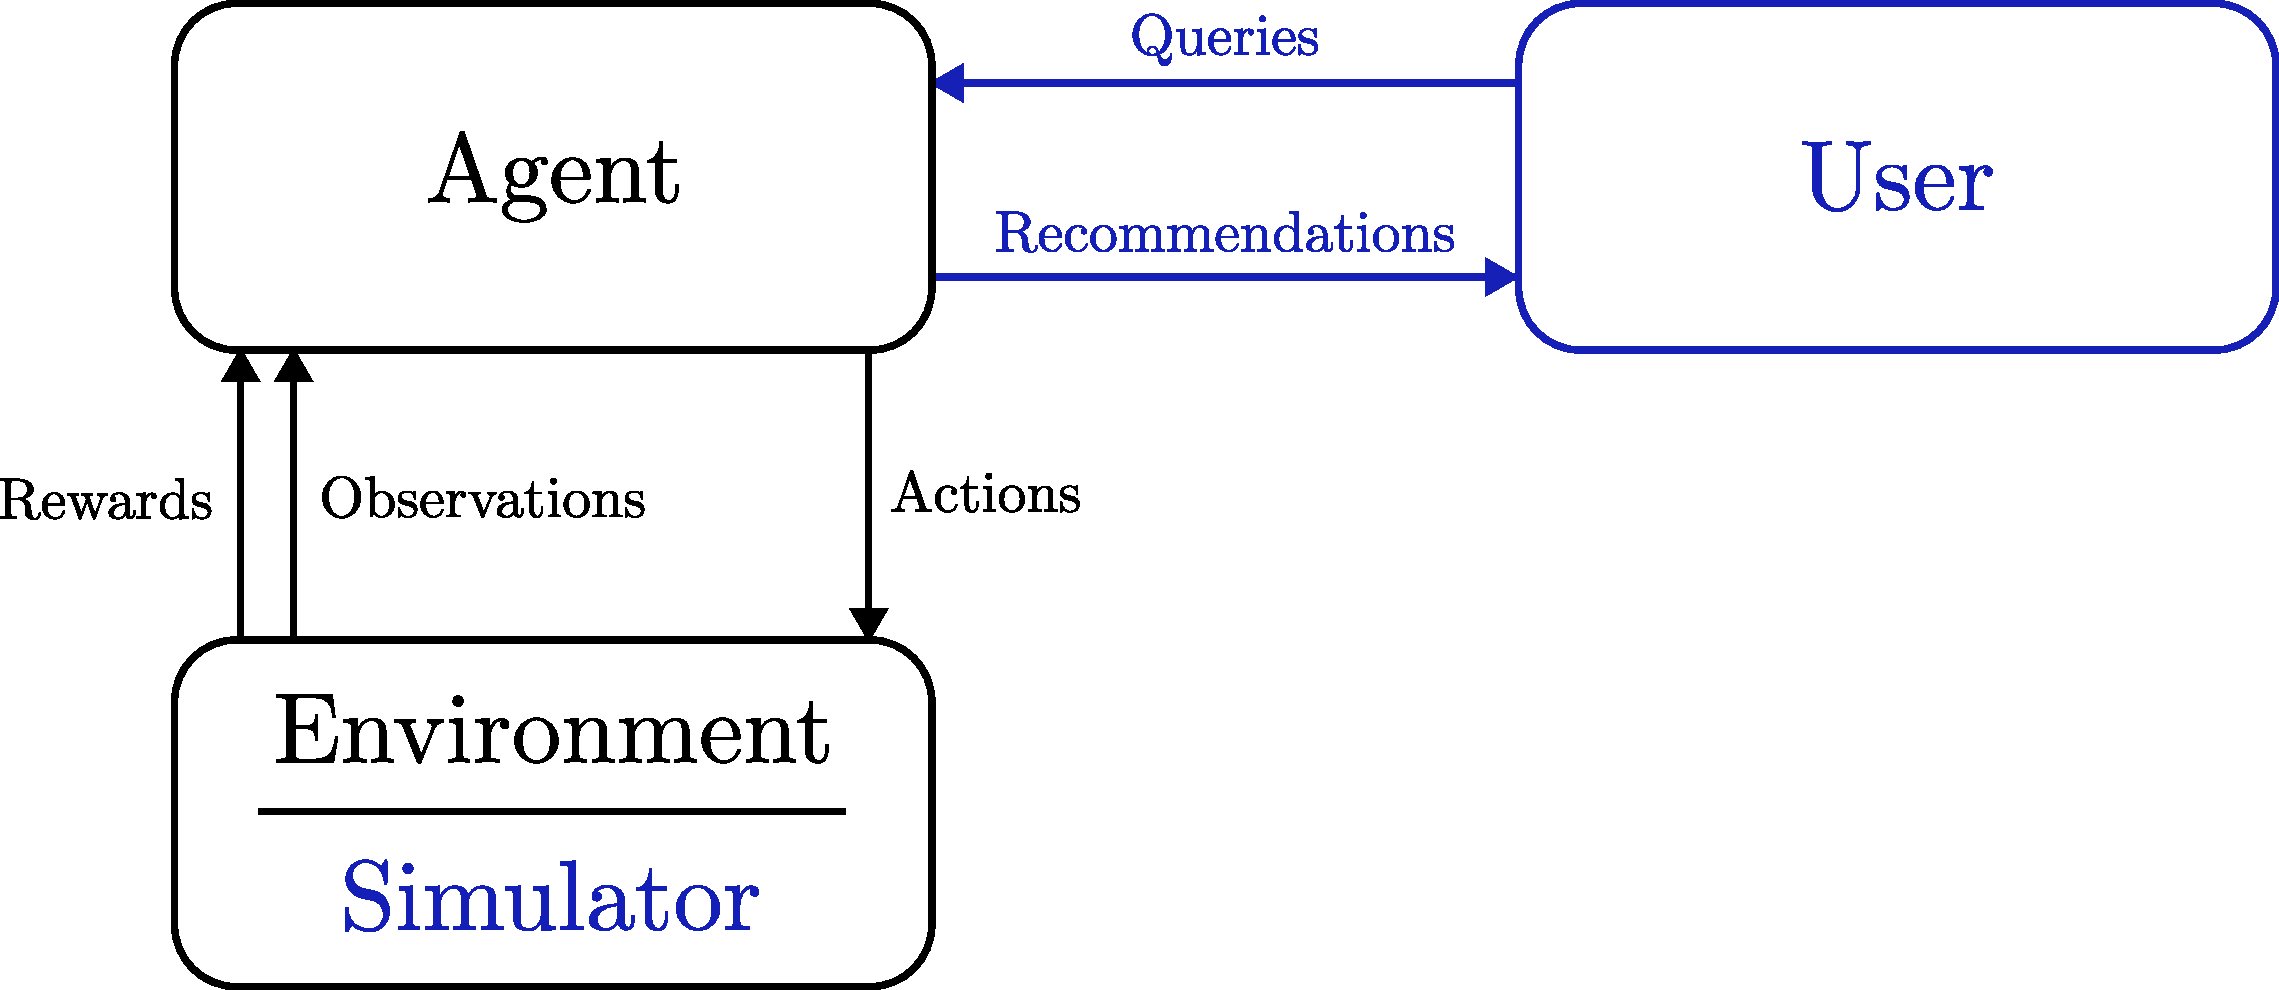
\includegraphics[width=0.75\textwidth]{figures/ch2/rl_overview.pdf} 
        \caption[Exploration setting in reinforcement learning.]{\todo{update fig to just be the blue version.} Exploration setting in reinforcement learning (\todo{reproduced and edited from fig 2.5}), \bd{where the agent aims to discover the optimal policy and has a larger emphasis on exploration to find better solutions rather than exploiting.}}
        \label{fig:4:rl_overview}
    \end{figure}

    Figure \ref{fig:4:rl_overview} gives the exploration setting for reinforcement learning, where the agent is only assessed on the recommendations that it provides, and is not penalised for considering poor actions in the simulator. 

    This chapter will also consider how entropuy can be used as an auxilary secondary objective to encourage exploration. Entropy is already used widely in the reinforcement literature \todo{cites, ppo, sac etc, ref ch3}, and is often cited for its \bd{exploration, and robustness to uncertainty, and robustness to simulator/environment differences, and robustness to noise.} 

    When considering the maximum entropy reinforcement learning objective (\todo{ref}), the optimal policy (equation (\todo{ref})) naturally takes the form of a Boltzmann policy. Notably, MENTS (Section \ref{sec:2-4-3-ments}), and RENTS and TENTS (Section \todo{ref litrev}) are existing MCTS algorithms for the maximum entropy setting (Section \ref{sec:2-3-1-merl}), so will be discussed further in this chapter, along with UCT (Section \todo{ref}), and used as baseline algorithms.

    Section \ref{sec:4-1-intro} discusses limitations of existing MCTS algorithms in this exploration setting, motivating the work covered in the remainder of the chapter. Additionally, the planning framework is defined so that the algorithms can be theoretically analysed using \textit{simple regret}.
    
    In Section \ref{sec:4-2-boltzmannsearch} the \textit{Boltzmann Tree Search} and \textit{Decaying ENtropy Tree Search} algorithms are defined.

    Section \ref{sec:4-3-toyenvs} considers some theoretical MDPs, which are used to empirically demonstrate the limitations of the existing MCTS algorithms, and are used for constructive proofs of some theorems. 

    Results on grid world and the game of Go are given in section \ref{sec:4-4-results}. 

    Finally, in Section \ref{sec:4-5-theory} the main theoretical analysis and proofs are given.

    \todo{add sect 4.6 if actually use that.}

    \todo{one paragraph for ch overview? Or make other descriptions longer? Or make it bullet points?}

    \todo{After finished writing, do another pass through neurips paper and check no results/writing missing from thesis that really should be included. (Thinking about some of the frozen lake plots in the appendix when writing this.)}
    







\section{Introduction and Motivation}
\label{sec:4-1-intro}

    UCT \todo{ref} \bd{is designed in the traditional reinforcement learning setting (todo ref Fig 2.5), minimising the cumulative regret (todo ref)}, and so UCT makes a trade off between exploration and exploitation. As such, UCT will frequently choose the same action to exploit, which results in it getting stuck in local optima when \bd{rewards are sparse or not informative.}

    To see this consider two grid world MDPs which differ only in the reward function. \todo{state space is (x,y,time), actions are cardinal directions etc}. The first reward function is to use a constant cost of $R_1(s,a)=-1$, and the second is a sparse version where the time cost is only revealed at the end $R_2((x,y,t),(x_a,y_a)) = -(t+1)\one[(x,y)+(x_a,y_a)==G]$. \todo{clean and actually define goal state, and name bettwer than R1 and R2}

    \todo{make diagram}

    \todo{something that says although this example can be solved by using the more sensible reward, it's just to highlight the issue of exploration}.
    
    \todo{would like to have figs showing the best path found by UCT in both cases AND showing the number of trials (one step of branches) where it explored.}

    Although the issues in the above toy problem can be resolved by using the simpler constant reward $R_1$, the example serves to highlight that UCT performs best when provided with a dense and informative reward. 
    
    As we are considering the exploration setting given in Figure \ref{fig:4:rl_overview}, this example shows in the sparse reward setting that UCT will use most of its available computation time exploiting the same sub-optimal solution that it has already found. As the objective is to provide the best recommendations to the user, it would be desirable to better utilise this computation time exploring alternative solutions. \todo{reword this sect, not super hapy with it }

    \todo{some comment somewhere that although it does seem a little unfair to compare UCT in a scenario for which it was not designed, in practise it is used in these cases}

    This example is extended upon in Section \todo{ref} where the performance of algorithms discussed in this chapter are compared on mixtures of these two rewards.





    Now that some limitations of UCT have been discussed, lets now consider the maximum entropy objective. When using the maximum entropy objective it is often argued that the standard objective can be recovered by setting $\alpha=0$, or setting $\alpha$ to an infitesimally small values ($0<\alpha<<1$). \todo{add refs} \todo{add the words ``temperature'' somewhere}

    However, in practise setting $\alpha$ to some tiny value will nullify any advantages that can be obtained from using entropy to promote exploration. Considering the other extreme, if we allowed a very large value of $\alpha$ (or let $\alpha\rightarrow\infty$), then maximising entropy becomes the dominant objective and the `optimal' policy will be a uniformly random one. Thus there is some tradeoff that needs to be made. When using a maximum entropy method the temperature parameter needs to be tuned: which intuitively should be made as large as possible, so as to obtain as much benefit from entropy exploration; while keeping it small enough such that policy acts as desired (i.e. it maximises the standard objective).

    \todo{supp expr on gridworld shortest path problem, where vary alpha value}

    In Figure \todo{ref}, the performance of MENTS (\todo{ref}) on the above gridworld problem with sparse reward is considered (Figure \todo{ref}). As the value of $\alpha$ is increased from zero, it can be seen the shortest path is found with fewer and fewer trials initially. Then, above a threshold value of \todo{quote value}, MENTS can gain more ``reward'' by acting randomly and optimising for entropy, largely ignoring the rewards from the MDP. This example empirically demonstrates an issue with using the maximum-entropy objective, where the temperature parameter needs to be finely tuned to a sweet-spot for it to be effective.

    More concretely, consider the policy $\pi_{\text{eval}}(s) = \argmax_{a'} \pi^*_{\sft}(a'|s)$ that would be followed at test time with the maximum entropy objective. In the following, the maximum entropy objective will be said to be \textit{misalligned} with the standard objective when $\pi_{\text{eval}}(s) \neq \pi^*(s)$.

    Building off this intuition, in Section \todo{ref}, an MDP is constructed such that the temperature parameter needs to be made prohibitively small (i.e. little to no benefit is gained from the entropy rewards) to avoid the maximum entropy objective from being missaligned.

    While only MENTS has been discussed, the issue lies predominantly from mixing entropy into the scalar objective, and as such similar issues arise no matter the form of entropy considered. \todo{basically saying RENTS and TENTS dont fix this problem}





    Now \textit{simple regret} is defined, which will be used motivate and analyse the algorithms developed. The simple regret of a policy is the difference between the value of the policy and optimal value of the policy (\todo{ref the equation below}). By definition, the optimal policy achieves a simple regret of zero, and an MCTS algorithm is considered \textit{consistent} if it's expected simple regret tends to zero. In plain english, an algorithm is consistent if left to run forever it would eventually output an optimal policy. An implication of consistency is that if an algorithm can be run for longer, then it is expected to improve on its solution.

    \todo{Talk about the setup we're using. Probably want to try motive similarly to DENTS paper, and recall the diagram from} \ref{sec:2-3-rl}. \todo{Say that in fig below that normally step 3 is not considered}

    \begin{figure}
        \begin{tcolorbox}
            Parameters: An MDP $\cl{M}$.
            \begin{itemize}
                \item For each round $m=1,2,...$:
                \begin{enumerate}
                    \item the agent produces a search policy $\pi^m$ to follow;
                    \item the environment samples a trajectory $\tau\sim\pi^m$ (including rewards $r_t=R(s_t,a_t)$ for each $s_t,a_t$ pair in $\tau$);
                    \item the agent produces a recommendation policy $\psi^m$;
                    \item if the environment sends a stop signal, then the game ends, otherwise the next round starts.
                \end{enumerate} 
            \end{itemize}
        \end{tcolorbox}
        \caption{The procedure of an exploring planning problem for MDPs. \todo{Make this sound better.} \todo{Also make ch2 MAB figs use enumerate?}}
        \label{fig:3:planning_problem}
    \end{figure}

    \todo{make this a proper def}
    Simple regret of a policy $\psi$ is then defined as
    \begin{align}
        \sreg(s,\psi) = V^*(s)-V^{\psi}(s).
    \end{align}

    \todo{make this a proper def}
    An agent, that produces recommendation policies $\psi^1,\psi^2,...$ is said to be \textit{consistent} if $\bb{E}[\sreg(s,\psi^m)] \rightarrow 0$ as $m\rightarrow \infty$.

    Returning to the discussion around UCT and MENTS now that simple regret and consistency has been defined. It can be shown the UCT is always consistent \todo{ref?}, although MDPs can be constructed where it requires a hyperexpontial amount of time to find the optimal policy. Whereas, the consistancy of MENTS depends on if the temperature parameter is sufficiently small for the optimal soft policy to not be misaligned with the standard optimal policy. Moreover, the threshold for the temperature parameter is dependent on the MDP, and so needs to be tuned on every MDP instance seperately.
    




    From the discussion in this section, the following properties are desired from the MCTS algorithms:
    \begin{itemize}
        \item define algorithms that are as simple to implement as UCT and MENTS;
        \item able to utilise dense and informative rewards (UCT \tick, MENTS \tick);
        \item effectively explore when rewards are sparse, or have sparse components (UCT \cross, MENTS \tick);
        \item are consistent, for parameters independent of the environment (UCT \tick, MENTS \cross). \todo{something like can get a reasonable result without haveing to tune params on each env. Maybe ``doesnt require parameter tuning on every environment''}
    \end{itemize}

    As such, this chapter will consider how entropy can be used as an additional secondary objective, while still focusing on performing well in the standard objective. \todo{place this better. Want it to say, that because the issue lies in the maximum entropy objective, we're going to start by stipping MENTS of the maximum entropy objective and then consider how it can be reintroduced in a consistent way.}









\section{Boltzmann Search}
\label{sec:4-2-boltzmannsearch}

    \todo{list}
    \begin{itemize}
        \item Recall MENTS
        \item Define BTS using THTS functions
        \item Define DENTS using THTS functions
        \item Discuss alias method variant (and complexity analysis) in a subsection?
    \end{itemize}

    \todo{would like to read more about the exp3 stuff before submitting this ch}
    \todo{https://tor-lattimore.com/downloads/book/book.pdf - bandits book}
    \todo{exp3 paper: http://rob.schapire.net/papers/AuerCeFrSc01.pdf}
    \todo{add to future work ideas to adapt BTS to use exp3 type stuff, and the thing gradient update covered in the Sutton and Barto book (todo get link and page ref to RL book where talk about that)}
    \todo{moved already}

    This section defines two algorithms Boltzmann Tree Search and Decaying ENtropy Tree Search in the \thtspp\ewe schema. 
    
    \subsection{Boltzmann Tree Search}
    \label{sec:4-2-1-bts}

        \todo{define BTS in thtspp}

        \todo{Define with variable alpha, change proofs to say for fixed alpha get regret bound. And add theorem that }


        Our first approach, put simply, replaces the use of soft values in MENTS with 
        % \textit{dynamic programming} (DP) 
        \textit{Bellman} 
        values. We call this algorithm \textit{Boltzmann Tree Search} (BTS).  The search policy $\pi_{\textnormal{BTS}}$ and backups for the $n$th trial are given by:
        %


        This section introduces the \textit{Boltzmann Tree Search} (BTS) algorithm, presented in terms of the \thtspp\ewe schema \todo{ref}. BTS promotes exploration through the stochastic Boltzmann search policy, like MENTS \todo{ref}, while using backups that optimise for the standard objective, like UCT \todo{ref}. Unlike MENTS, the temperature parameter generalised to a function $\alphabts(x) > 0$, which allows the temperature to vary with the number of times that a node has visited. BTS uses Bellman value estimates at each node $\Vbts$ and $\Qbts$. The search policy is defined by:
        %
        \begin{align}
            \pibts(a|s) &= (1-\lambdabts)\rhobts(a|s) + \frac{\lambdabts}{|\cl{A}|}, 
                        \label{eq:4:bts_search_policy} \\ 
            \rhobts(a|s) &\propto \exp\left(\frac{1}{\alphabts(N(s))}\left(\Qbts(s,a)\right)\right).
                        \label{eq:4:bts_value_policy} \\
            \lambda(s,x) &= \min\left(1, \frac{x}{\log(e+N(s))}\right) \label{eq:4:lambda}
        \end{align}
        %
        where $\epsbts \in (0,\infty)$ is an exploration parameter and $\alphabts(x)$ is the search temperature schedule. \todo{Add a comment about defining rho as taking the max when N(s) is zero?} And given a trajectory $\tau=(s_0,a_0,r_0,...,s_{h-1},a_{h-1},r_{h-1},s_h)$ the value estimates are updated for $t=h-1,...,0$:
        \begin{align}
            \Qbts(s_t,a_t) &\leftarrow 
                R(s_t,a_t) + \sum_{s' \in \suc{s_t}{a_t}} \left( \frac{N(s')}{N(s_t,a_t)} \Vbts(s') \right), 
                        \label{eq:4:bts_backup_q} \\ 
            \Vbts(s_t) &\leftarrow \max_{a\in\cl{A}} \Qbts(s_t,a).
                        \label{eq:4:bts_backup_v} 
        \end{align}
        
        In line with the \thtspp\ewe schema, the values of $\hat{V}_{\bts}(s)$ and $\hat{Q}_{\bts}(s,a)$ are initialised using the arbitrary functions $\Vinit$ and $\Qinit$, which for example can be set to a constant value or be the output from a neural network. \todo{check all of the above definition is in line with thtspp definition} 
        
        
        When BTS needs to recommend a policy, it can use it's Q-value estimates:
        %
        \begin{align}
            \psibts(s)=\argmax_{a\in\cl{A}}\Qbts(s,a).
        \end{align}
        %
        Alternatively, the node visit counts can be used in the recommendation policy
        \begin{align}
            \mvbts(s) = \argmax_{a\in\cl{A}} N(s,a).
        \end{align}
        %
        \todo{Find better notation for this?}

        As BTS uses Bellman backups, it can be guaranteed that the BTS recommendation policy converges to the optimal standard policy. \todo{make this sound better given we're also talking about most visited recommendation policy now.}
        








        \todo{Work out how best to add the AR-BTS stuff?}

        Additionally, this search policy can still be used with average returns. The following is a summary of the definitions for \textit{Boltzmann Tree Search with Average Returns} (AR-BTS), which uses the value estimates of $\Varbts$ and $\Qarbts$ at each node, and temperature schedule $\alphaarbts(x) > 0$:
        %
        \begin{align}
            \piarbts(a|s) &= (1-\lambdaarbts)\rhoarbts(a|s) + \frac{\lambdaarbts}{|\cl{A}|}, 
                        \label{eq:arbts_search_policy} \\ 
            \rhobts(a|s) &\propto \exp\left(\frac{1}{\alphaarbts(N(s))}\left(\Qarbts(s,a)\right)\right).
                        \label{eq:arbts_value_policy}
        \end{align}
        %
        where $\epsarbts \in (0,\infty)$ is an exploration parameter and $\alphaarbts(x)$ is the search temperature schedule. Given a trajectory $\tau=(s_0,a_0,r_0,...,s_{h-1},a_{h-1},r_{h-1},s_h)$ and the leaf node value estimate $\tilde{r} = \Vinit(s_h)$, the value estimates are updated for $t=h-1,...,0$:
        \begin{align}
            \Qarbts(s_t,a_t) &\leftarrow 
                \frac{1}{N(s_t,a_t)} \left( (N(s_t,a_t)-1) \Qarbts(s_t,a_t) 
                    + \tilde{r} + \sum_{i=t}^{h-1} r_i \right) \label{eq:4:arbsts_backup_q} \\
            \Varbts(s_t) &\leftarrow 
                \frac{1}{N(s_t)} \left( (N(s_t)-1) \Varbts(s_t) 
                    + \tilde{r} + \sum_{i=t}^{h-1} r_i \right). \label{eq:4:arbsts_backup_v} 
        \end{align}

        Similarly to BTS, either the Q-value estimates can be used for a recommendation policy or the most visited child node can be used:
        \begin{align}
            \psiarbts(s) &= \argmax_{a\in\cl{A}}\Qbts(s,a), \\
            \mvarbts(s) &= \argmax_{a\in\cl{A}} N(s,a).
        \end{align}
        %
        \todo{Still find better notation for this?}








        In Section \todo{ref} convergence results about BTS and AR-BTS are given, which are summarised below:
        %
        \begin{itemize}
            \item BTS is consistent and converges for any setting of parameters;
            \item if $\alphabts(x) \geq L > 0$: BTS converges with an theoretical exponential rate;
            % \item if $\alphabts(x) \rightarrow 0$: BTS converges still;
            \item if $U \geq \alphaarbts(x)$ and $\alphaarbts(x) \rightarrow 0$: AR-BTS converges;
        \end{itemize}
        %
        noting that these results are independent of all of the other parameters, including which of the two recommendation policies are used.

        \todo{Add theorems here? Or just reference theorems?}

        \todo{Is the upper bound needed for arbts? Revisit these after having written the proofs up.}








        % By using Bellman backups, we can guarantee that the BTS recommendation policy converges to the optimal standard policy for any temperature $\alpha$, given enough time. In other words, BTS is consistent.
        % %
        % \begin{theorem} 
        %     \label{thrm:bts}
        %     For any MDP $\cl{M}$, after running $n$ trials of the BTS algorithm with a root node of $s_0$, there exists constants $C,k>0$ such that for all $\varepsilon>0$ we have $\bb{E}[\sreg(s_0,\psibts)] \leq C\exp(-kn)$, and also $\Vbts(s_0) \rap V^*(s_0)$ as $n\rightarrow\infty$.
        % \end{theorem}

        % \todo{update for $\alpha$ being const etc. Add the more theorems about BTS here.}
        % \begin{proofoutline}
        % 		This result is a special case of Theorem \ref{thrm:dents} by setting $\beta(m)=0$.
        % \end{proofoutline}
        % \begin{proof}
        %     Proofs for Theorem \ref{thrm:bts} and Theorem \ref{thrm:dents} provided in Appendix \ref{app:proofs}.
        % \end{proof}






    
    \subsection{Decaying ENtropy Tree Search}
    \label{sec:4-2-2-dents}

        \todo{add label}
        \todo{define DENTS in thtspp}

        \textit{Decaying ENtropy Tree Search} (DENTS) extends the BTS algorithm by introducing \textit{entropy estimates}. In DENTS nodes have a secondary entropy value estimate, $\HVdents$ and $\HQdents$, which are monte carlo estimates the entropy of the search policy rooted from the relevant node. By keeping a separate estimate for entropy, DENTS is able to use entropy in it's search policy, and discard it for recommendations.

        Given a trajectory $\tau=(s_0,a_0,r_0,...,s_{h-1},a_{h-1},r_{h-1},s_h)$, the entropy values are updated as follows for $t=h-1,...,0$:
        \begin{align}
            \HVdents(s_t) &\leftarrow \cl{H}(\pidents(\cdot | s_t)) + \sum_{a\in\cl{A}} \pidents(a|s_t)\HQdents(s_t,a), 
            \label{eq:4:dents_entropy_v_backup} \\
            \HQdents(s_t,a_t) &\leftarrow \sum_{s'\in \suc{s_t}{a_t}} \frac{N(s')}{N(s_t,a_t)} \HVdents(s'), 
            \label{eq::4dents_entropy_q_backup}
        \end{align}
        %
        where $\cl{H}$ is the Shannon entropy function. \todo{sentence about how the entropy values are initialised} $\HVdents(s) \leftarrow 0$.

        The entropy values are used as an exploration bonus in the search policy, and are weighted by a non-negative function $\betadents(x)\geq 0$. Generally this will be set to a function such that $\betadents(x)\rightarrow 0$ as $x\rightarrow\infty$ and will achieve better theoretical performance in this case. The DENTS search policy $\pidents$ is defined follows:
        %
        \begin{align}
            \pidents(a|s) &= (1-\lambdadents)\rhodents(a|s) + \frac{\lambdadents}{|\cl{A}|}, 
                        \label{eq:dents_search_policy} \\ 
            \rhodents(a|s) &\propto \exp\left(\frac{1}{\alphadents(N(s))}\left(\Qdents(s,a)+\beta(N(s))\HQdents(s,a)\right)\right).
                        \label{eq:dents_value_policy}
        \end{align}

        And finally, given the the trajectory $\tau$ the Bellman value estimates for DENTS, $\Vdents$ and $\Qdents$ are updated identically to BTS for $t=h-1,...,0$:
        \begin{align}
            \Qdents(s_t,a_t) &\leftarrow 
                R(s_t,a_t) + \sum_{s' \in \suc{s_t}{a_t}} \left( \frac{N(s')}{N(s_t,a_t)} \Vbts(s) \right), 
                        \label{eq:dents_q_backup} \\ 
            \Vdents(s_t) &\leftarrow \max_{a\in\cl{A}} \Qbts(s_t,a), 
                        \label{eq:dents_v_backup} 
        \end{align}

        \todo{also give the recommendation policies}

        




        \todo{Write about AR-DENTS here? My brain is getting bored copying and slightly editing things. this is just copying dents and then copying the value backups from ar-bts}






        Section \todo{ref} also provides convergence results about DENTS and AR-DENTS are given, which are summarised below:
        %
        \begin{itemize}
            \item When using the \todo{default? Bellman?} recommendation policy:
            \begin{itemize}
                \item DENTS is consistent and converges for any setting of parameters;
                \item if $\alphadents(x) \geq L > 0$: DENTS converges with an theoretical exponential rate;
                \item if $U \geq \alphaardents(x)$ and $\alphaarbts(x) \rightarrow 0$: AR-BTS converges;
            \end{itemize}
            \item When using the most visited recommendation policy, the same results hold, but additionally requires $\betadents(x)\rightarrow 0$.
        \end{itemize}

        \todo{Add theorems here? Or just reference theorems?}

        \todo{Double check these after having written up the proofs. Particularly the differences between using the two different recommendation policies.}









    \subsection{Advantages of Stochastic Search Policies}
    \label{sec:4-2-3-stoch_search_policies}

        Using a stochastic search policy in MCTS (or \thtspp) provides more benefits than just encouraging exploration through randomly sampled actions. In particular, the Alias Method (Section \ref{sec:2-6-sampling}) can be used to trade off using the most up to date policy for computational speed. Moreover, when prior knowledge (in the form of a policy prior) is available \todo{cite alphago etc}, it can naturally be integrated into the search using a \textit{mixture policy}.

        \todo{add ref to} \complexityq






        \subsubsection{The Alias Method in MCTS}

        When using the Alias Method in \thtspp\ewe an alias table \todo{capitalise?} is constructed at every decision node. This table can be updated every $\lambda|\cl{A}|$ visits to the node, for an arbitrary $\lambda\in\bb{R}_{>0}$, giving an amortised complexity of $O(1)$. \todo{just say constant amortised complexity?} $O(O(1)+\frac{|\cl{A}}{\lambda|\cl{A}|}) = O(O(1)+\frac{1}{\lambda}) = O(1)$. \todo{probably dont need to do that maths.} In \thtspp the value of the $\lambda$ can be varied to adjust the trade off between The value of lambda can be varied to adjust the trade off between up-to-dateness and sampling speed. For the remainder \todo{find a better way of saying this}, $\lambda=1$ will be considered \todo{but all of the results still hold}. Note that when a new decision node is constructed and added to the tree, there will still be a cost of $O(|\cl{A}|)$ to construct the new alias table.
        
        Although this will always lead to quite a significant computational speedup, in the case where \mctsmode, the computational speedup is also asymptotic. \todo{where this paragraph go?}

        In the following, the computational complexity to run $n$ trials is considered.
        
        First consider the computational complexity of running UCT: at each decision node visited on a trial, the maximum over $|\cl{A}|$ values is computed \todo{this is worded poorly}, on each trial at most $H_{\thtspp}$ decision nodes will be visited. Hence, the computational complexity of running $n$ trials of UCT is $O(nH_{\thtspp}|\cl{A}|)$.

        \todo{copy out appendix C stuff, cleaning up above and below as needed}

        Finally, considering the case when \thtspp\ewe is not running in \mctsmode, the asymptotic complexity is still $O(nH_{\thtspp}|\cl{A}|)$, as each trial is sampled until the planning horizon $H_{\thtspp}$ 

        \todo{Talk about co}

        \todo{add label}
        \todo{write about alias sampling}


        






        \subsubsection{Encorporating Prior Knowledge Through Mixture Policies}

        Let $\pi$ be some \thtspp\ewe search policy, and supposed that we have access to another policy $\tilde{\pi}$ with prior knowledge, such as a neural network. Then a new search policy $\pi_{\text{mix}}$ can be naturally be defined using a mixture of $\pi$ and $\tilde{\pi}$.

        \todo{some comment about just using the same mixing function as before ... because? .. it lets it tend towards the correct thing}

        The mixture policy is defined by:
        \begin{align}
            \pi_{\text{mix}}(a|s) = 
                (1-\lambda(s,\epsilon_{\text{mix}})) \pi(a|s) 
                + \lambda(s,\epsilon_{\text{mix}}) \tilde{\pi}(a|s),
        \end{align}

        where $\lambda$ is the same function as defined in equation (\todo{ref}), and $\epsilon_{\text{mix}}\in(0,\infty)$ weights the amount to use the prior knowledge by. \todo{word better}.

        \todo{are there theoretical results? Maybe we can show that for arbitrary function that it doesnt change anything. It should be the same as mixing in the uniform. Also another good reason to use the same function, because then the proof is basically the same thing as before.}


        
        \todo{write about using $\tilde{\pi}$, $\tilde{Q}$, $\tilde{V}$?}
        \todo{talk about grid world and how Qinit need to be able to handle costs}

        \todo{discuss the MENTS intiialisation here? :} MENTS suggests using $\tilde{\pi}$ as \todo{their description}
        %
        However, this may still lead to issues in for example in grid world problems. \todo{talk about }









    \subsection{Things still missing in this section}
        Defining the average reward versions of the algorithms

        \todo{Talking about the OG DENTS algorithm and why that didn't work? I feel like its a reasonable question}







\section{Toy Environments}
\label{sec:4-3-toyenvs}

    \todo{list}
    \begin{itemize}
        \item Define D-chain stuff from the paper
        \item Define the D-chain with entropy trap
        \item Front load some results still
    \end{itemize}

    \todo{(commented out below this), original writing in the motivation section, which talked about the d-chain environment.}

    % In the maximum entropy objective, it is argued that the standard objective can be recovered by setting $\alpha=0$ or setting $\alpha$ infitesimally small ($0<\alpha<<1$). \todo{add quote}. 
    % %
    % \todo{Although this is theoretically true (TODO ref the result about MENTS), in practise it is desirable to use the largest temperature that doesn't lead to undesirable (random) behaviour. In other words, extermely small temperatures do not utilise entropy for exploration effectively, while extremely large temperatures encourage agents to act randomly rather (reword: optimise for the standard objective). MENTS is used in (TODO) to demonstrate this issue with the maximum-entropy objective empirically, and (TODO) provides a corresponding theoretical result around MENTS.}
    % %
    % Although this is true, the most benefit can be gained from using entropy as an exploration bonus by setting a larger value of $\alpha$. This is highlighted in Figure \todo{ref}, where the performance on MENTS on the modified D-chain environment can be seen to improve as $\alpha$ is made larger, until a sudden drop off when it surpasses a threshold (\todo{at the poing 0.142ish}).
     
    % Above the threshold, an agent can gain more ``reward'' by acting randomly and optimising for maximum-entropy, largely ignoring the rewards of the MDP. This example demonstrates an issue with using the maximum-entropy objective, where the temperature parameter needs to be finely tuned to a sweet-spot for it to be effective.

    % This issue can be exasurbated further by editing the D-chain environment to contain an entropy trap. In the entropy trap environment \todo{ref fig}, an additional trap for maximum-entropy agents is added to the D-chain environment. In this environment, when the end of the chain is reached, there are two choices, to either collect the immediate reward of $1$, or to follow another path where high entropy can be obtained, but no reward can be obtained. The maximum entropy that can be obtained from following the chain is $\alpha K \log(2)$, and as such will mislead any maximum-entropy agents that have a temperature parameter of $\alpha > \frac{1}{k\log(2)}$. Setting \todo{k=what}, sets this threshold at \todo{todo say $\alpha > C$ for now}. However, for $\alpha \leq C$, the temperature parameter is low enough that not much benefit is gained from the entropy objective.

    % Figure \todo{ref} shows the performance of ments on the entropy trap environment, highlighting that it doesn't perform well for any setting of $\alpha$. In contrast, the algorithms defined in this chapter are able to overcome these issues.

\section{Empirical Results}
\label{sec:4-4-results}

    \todo{list}
    \begin{itemize}
        \item DChain
        \item GridWorlds
        \item Go
    \end{itemize}

    - Get some better results using hyperparam optimise
    - want a dense env where the (not entropy) temp decay fn gets optimised to soemthing that decays a lot
    - want a sparse env where the temp decay fn gets optimised to something flat (or basically flat)

    \todo{ TWO: would like to have experiments which vary the proportion of the sparse reward. So have FL(lambda), where lambda specifies the ratio between the dense and sparse rewards. Then investigate what happens as vary lambda. So this is the grid world experiments run again, }

\section{Theoretical Results}
\label{sec:4-5-theory}

    \todo{list}
    \begin{itemize}
        \item add theoretical results
    \end{itemize}

    Should we try to add a result about most visited? Where will be concentration bounds around the number of visits being proportional to the values. So think can bootstrap those proofs.

    - Generalise the AR proof to say that for decaying search functions still work (as long as they are bounded)
    - Have a result that using most visited is theoretically sound

    The Neurips paper proof section was structured as follows:
    \begin{enumerate}
        \item First, in Section \ref{app:mcts_process} we revisit MCTS as a stochastic process, defining some additional notation that was not useful in the main body of the paper, but will be for the following proofs;
        \item Second, in Section \ref{app:preliminaries} we introduce preliminary results, that will be useful building blocks for proofs in later Theorems;
        \item Third, in Section \ref{app:soft_learning_results} we show some general results about soft values that will also be useful later;
        \item Fourth, in Section \ref{app:simple_regret_results} simple regret is then revisited, and we show that any bounds on the simple regret of a policy are equivalent to showing bounds on the simple regret of an action;
        \item Fifth, in Section \ref{app:q_result} we show in a general way, that if a value function admits a concentration inequality, then the corresponding Q-value function admits a similar concentration inequality;
        \item Sixth, in Section \ref{app:ments_results} we show concentration inequalities for MENTS about the optimal soft values, and give bounds on the simple regret of MENTS, provided the temperature parameter is sufficiently small;
        \item Seventh, in Sections \ref{appsec:dents_proofs} and \ref{appsec:bts_proofs} we also provide concentration inequalities around the optimal standard values for BTS and DENTS, and give simple regret bounds, irrespective of the temperature paramters;
        \item Finally, in Section \ref{sec:ar_proofs} we consider results that are relavant for the algorithms using average returns from Section \ref{app:average_returns}.
    \end{enumerate}

    \todo{above is note taking and below is me starting to write the proofs stuff}













%%%%
% THEORY - Stochastic Processes Definitions
%%%%



\todo{Some comment about using a policy of the form XXX will be refered to a Boltzmann MCTS Process.}



\subsection{MCTS As A Stochastic Process}
    Now the MENTS, BTS and DENTS are written as a stochastic process, where values are indexed (with a superscript) by the number of times that the corresponding node has been visited. For completeness and reference, the stochastic processes for \todo{UCT?}, MENTS, BTS and DENTS are given below.
    


    \todo{change m to n, and use mth when need to reason about prev trials (whole subsection)}

    When reasoning about a \textit{MCTS stochastic process} the following notations will be helpful.
    \begin{itemize}
        \item 
            The search policy used on the $m$th trial is $\pi^m$, and if the process were stopped after $m$ trials, the recommendation policy that the algorithm would output is denoted $\psi^m$. Where if the process is run for $n$ trials, then $m$ ranges from $1$ to $n$.
        \item 
            The $m$ trajectory sampled is $\tau^m=(s_0^m,a_0^m,...,s_{h-1}^m,a_{h-1}^m,s_{h}^m)$ \todo{add reward, also make it h subscript m instead of h?}, and is sampled using the search policy $\tau^m \sim \pi^m$ (that is $a^m_i \sim \pi^m(\cdot|s^m_i)$ and $s^m_{i+1} \sim p(\cdot | s^m_i, a^m_i)$). \todo{comment that $k$th trial is run until h where s subscript h is termal in some thtspp sense. Comment about how the superscripts on s a and r will be used when necessary, but not always}
        \item 
            The search tree after $m$ trials is denoted $\cl{T}^m$, the initial search tree is $\cl{T}^0=\{s_0\}$, and $\cl{T}^k = \cl{T}^{k-1} \cup \tau^k$.
    \end{itemize}

    When making arguments that apply to multiple algorithms the general policies $\pi$ and $\psi$ will be used, and when making arguments about specific algorithms the subscripts will be used, such as $\pibts$. Note that superscript is used to index with respect to the trial, and superscript with parenthasis is used to denote the number of visits.

    In the proofs of following sections, it will be useful to write the number of times state~$s$ was visited in the first $m$ trials as $N(s,m)$, and the number of times action~$a$ was selected from state~$s$ in the first m trials as $N(s,a,m).$ Additionally, it will be useful to write these quantities in terms of indicator random variables. 
    
    Let $T(s_t,m)$ (and $T(s_t,a_t,m)$) be the set of trajectory indices that $s_t$ was visited on (and action $a_t$ selected) in the first $m$ trials, that is: \todo{this can avoid using s subscript t}
    %
    \begin{align}
        T(s_t,m) &= \{i | i\leq m, s^i_t = s_t \} \\
        T(s_t,a_t,m) &= \{i | i\leq m, s^i_t = s_t, a^i_t = a_t \}.
    \end{align}
    %
    This allows the counts $N^m(s_t),$ $N^m(s_t,a_t)$ and $N^m(s_{t+1})$ (with $s_{t+1}\in\suc{s_t}{a_t}$) to be written as sums of indicator random variables in the following ways:
    %
    \begin{align}
        N(s_t,m) &= \sum_{i=1}^m \one[s^i_t=s_t] = |T(s_t,m)|, \\
        N(s_t,a_t,m) &= \sum_{i=1}^m \one[s^i_t=s_t,a^i_t=a_t] = |T(s_t,a_t,m)|, \\ 
        N(s_t,a_t,m) &= \sum_{i\in T(s_t,m)} \one[a^i_t = a_t], \label{appeq:nsa_sum} \\
        N(s_{t+1},m) &= \sum_{i\in T(s_t,a_t,m)} \one[s^i_{t+1} = s_{t+1}]. \label{appeq:ns_sum}
    \end{align}
    %
    Additionally, the assumption that for any two states $s,s'\in\cl{S}$ \todo{double check use calligraphic S for state space?} that $s=s'$ if and only if the trajectories leading to them are identical is made. This assumption is purely to simplify notation, so that nodes in the tree have a one-to-one correspondence with states (or state-action pairs). \todo{move this up}
        
        
        
        

    \todo{do we do anything at all with the UCT process?}
    % \subsubsection{The UCT process.} 
    % 	The UCT search policy can be defined as:
    % %
    % \begin{align}
    %      \pi_{\textnormal{UCT}}^n(s_t) &= \max_{a\in\cl{A}} \text{UCB}^n(s_t,a), \\
    %      \text{UCB}^n(s_t, a) &= 
    %     		\begin{cases}
    %     			\infty & \text{if } N(s_t,a)=0 \\
    %     			\bar{Q}^{N(s_t,a)}(s_t, a)+c \sqrt{\frac{\log N(s_t)}{N(s_t, a)}} & \text{if } N(s_t,a)>0
    %     		\end{cases}
    % \end{align}
    % %
    % \noindent where, after $n$ trials, $\bar{Q}^{N(s,a)}(s,a)$ is the empirical estimate of the value at node $(s,a)$, where action~$a$ has been selected $N(s, a)$ from state~$s$. The backup consists of updating empirical estimates for $t=h-1,...,0$:
    % %
    % \begin{align}
    %     \bar{V}^{N(s_t)+1}(s_t) &= \bar{V}^{N(s_t)}(s_t) + \frac{\bar{R}(t) - \bar{V}^{N(s_t)}(s_t)}{N(s_t) + 1}, \label{appeq:uct_vbar} \\
    %     \bar{Q}^{N(s_t,a_t)+1}(s_t, a_t) &= \bar{Q}^{N(s_t,a_t)}(s_t, a_t) + \frac{\bar{R}(t) - \bar{Q}^{N(s_t,a_t)}(s_t, a_t)}{N(s_t, a_t) + 1}, \label{appeq:uct_qbar}
    % \end{align}
    % %
    % \noindent where $\bar{R}(t) = V^{\text{init}}(s_h) + \sum_{i=t}^{h-1} R(s_i,a_i)$, and values are initialised as $\bar{V}^1(s)=V^{\text{init}}(s)$ and $\bar{Q}^0(s,a)=0$. 
    

    
    
    
    \subsubsection{The MENTS Process}
    
    Below is a complete summary of the MENTS process, for reference. On the $m$th trial, the MENTS process follows the search policy:

    \todo{make ments section in ch2 use consistent definitions of alphaments, lambdaments and so on}

    \begin{align}
        \mpiments{m}(a|s) &= (1-\mlambdaments{m})\mrhoments{m}(a|s) + \frac{\mlambdaments{m}}{|\cl{A}|}, 
                    \label{appeq:ments_soft_policy} \\ 
        \mrhoments{m}(a|s) &= \exp\left(
            \frac{1}{\alphaments}\left(\mQments{N(s,a,m-1)}(s,a)-\mVments{N(s,m-1)}(s)\right)\right). \\
        \lambda^m(s,x) &= \min\left(1, \frac{x}{\log(e+N(s,m-1))}\right),
    \end{align}
    %
    where $\epsments\in(0,\infty)$ is an exploration parameters, and $\alphaments$ is the temperature parameter. 

    The $m$th trajectory is sampled using the search policy: $\tau^m \sim \piments^m$. Letting $\tau^m=(s_0,a_0,r_0,...,s_{h-1},a_{h-1},r_{h-1},s_{h})$, the MENTS value estimates are computed using backups for $t=h-1, ..., 0$: \todo{either add the superscript m into every s and a, or update words to say implicit}
    \begin{align}
        \mVments{N(s_t,m)}(s_t) &= 
            \alphaments \log \sum_{a\in\cl{A}} \exp \left(
                \frac{1}{\alphaments}\mQments{N(s_t,a,m)}(s_t,a) \right), \label{appeq:soft_v_backup} \\
        \mQments{N(s_t,a_t,m)}(s_t,a_t) &= 
            R(s_t,a_t) + \sum_{s'\in\suc{s}{a}} \left( 
                \frac{N(s',m)}{N(s_t,a_t,m)} \mVments{N(s',m)}(s') \right). \label{appeq:soft_q_backup}
    \end{align}

    \todo{also want something about initialisation and everything in line with thtspp}
    %
    % The soft (Q-)values are initialised as $\Vst{s}{1}=V^{\text{init}}(s)$ and $\Qst{s}{a}{0}=Q^{\text{init}}_{\sft}(s)$ (typically $Q^{\text{init}}_{\sft}(s)=0$).

    \todo{recommendation policies and some comment about it being the soft values used?}
    \begin{align}
        \mpsiments{m}(s) &= \argmax_{a\in\cl{A}}\mQments{N(s,a,m)}(s,a), \\
        \mmvments{m}(s) &= \argmax_{a\in\cl{A}} N(s,a,m).
    \end{align}










\subsubsection{The DENTS Process}

    \todo{this whole sections math is pretty mess and a struggle to fit onto one line at a time. Maybe it suffices to just wordily describe the values of the sufixed values?}

    Follow policy: 
    %
    \todo{add more wordy things. Some things we said here before were: (1) defining beta} $\beta : \bb{R}\rightarrow [0,\infty)$ be a bounded function; \todo{(2) defined epsilon as exploration policy; (3) in Neurips we defined the propto version of rho and also the full version saying ``becasue we need to reason about the search policy we give the exact form,'' for the moment I've kept both. I think just copy the full version where relevent in the proofs.}
    %
    \begin{align}
        \mpidents{m}(a|s) &= (1-\mlambdadents{m})\mrhodents{m}(a|s) + \frac{\mlambdadents{m}}{|\cl{A}|}, 
            \label{appeq:dents_search_policy}  \\
        \mrhodents{m}(a|s) &\propto \exp\left(\frac{1}{\alphadents(N(s,m))}
            \left(\mQdents{N(s,a,m-1)}(s,a) + \betadents(N(s,m))\mHQdents{N(s,a,m-1)}(s,a) \right)\right). \\
        \mrhodents{m}(a|s) &= \frac{
            \exp\left(\frac{1}{\alphadents(N(s,m))}\left(
                \mQdents{N(s,a,m-1)}(s,a) + \betadents(N(s,m))\mHQdents{N(s,a,m-1)}(s,a)   \right)\right)
            }{\sum\limits_{a'\in\cl{A}} \exp\left(\frac{1}{\alphadents(N(s,m))}\left(
                \mQdents{N(s,a',m-1)}(s,a') + \betadents(N(s,m))\mHQdents{N(s,a',m-1)}(s,a')  \right)\right)}.  
            \label{appeq:full_rho} \\
        \lambda^m(s,x) &= \min\left(1, \frac{x}{\log(e+N(s,m-1))}\right), 
    \end{align}

    The $m$th trajectory is sampled using the search policy: $\tau^m \sim \piments^m$. Letting $\tau^m=(s_0,a_0,r_0,...,s_{h-1},a_{h-1},r_{h-1},s_{h})$, the DENTS value and entropy estimates are computed using backups for $t=h-1, ..., 0$: \todo{either add the superscript m into every s and a, or update words to say implicit}
    \begin{align}
        \mQdents{N(s_t,a_t,m)}(s_t,a_t) &= 
            R(s_t,a_t) + \sum_{s' \in \suc{s_t}{a_t}} \left( 
                \frac{N(s',m)}{N(s_t,a_t,m)} \mVdents{N(s',m)}(s') \right), 
            \label{appeq:dp_q_backup} \\ 
        \mVdents{N(s_t,m)}(s_t) &=\max_{a\in\cl{A}} \mQdents{N(s_t,a,m)}(s_t,a), 
            \label{appeq:dp_v_backup} \\
        \mHQdents{N(s_t,a_t,m)}(s_t,a_t) &= 
            \sum_{s'\in \suc{s_t}{a_t}} \frac{N(s',m)}{N(s_t,a_t,m)} \mHVdents{N(s',m)}(s'), \\
        \mHVdents{N(s_t)}(s_t) &= 
            \cl{H}(\mpidents{m}(\cdot | s_t)) 
                + \sum_{a\in\cl{A}} \mpidents{m}(a_t|s_t)\mHQdents{N(s_t,a_t,m)}(s_t,a_t).
    \end{align}

    \todo{also want something about initialisation and everything in line with thtspp}
    %
    % The (Q-)values are initialised as $\Vt{s}{1}=V^{\text{init}}(s)$ and $\Qt{s}{a}{0}=Q^{\text{init}}_{\sft}(s)$ (typically $Q^{\text{init}}_{\sft}(s)=0$). The entropy values are initialised as $\cl{H}_Q^{0}(s,a)=0$ and $\cl{H}_V^{1}(s) = \cl{H}(\pi^n_{\text{DENTS}}(\cdot | s_t))$, where the node for $s$ is created on the $n$th trial

    \todo{recommendation policies word stuff}
    \begin{align}
        \mpsidents{m}(s) &= \argmax_{a\in\cl{A}}\mQdents{N(s,a,m)}(s,a), \\
        \mmvdents{m}(s) &= \argmax_{a\in\cl{A}} N(s,a,m).
    \end{align}

    \todo{From the neurips, also wrote the following (everything left in this subsubsection is copied and cleaned up, but probably needs a proof read)} Let $\mVrhodents{N(s)}(s)$ be defined as the value:
    %
    \begin{align}
        \mVrhodents{N(s)}(s) = &
            \alphadents(N(s,m)) \log \Bigg[ \sum_{a'\in\cl{A}} \exp\bigg(\frac{1}{\alphadents(N(s,m))}
                \big(\mQdents{N(s,a')}(s,a') \nonumber \\
            &+ \betadents(N(s,m))\mHQdents{N(s,a')}(s,a') \big)\bigg)\Bigg], \label{appeq:v_rho}
    \end{align} 
    %
    and notice that the value of $\exp(\mVrhodents{N(s,m)}(s)/\alphadents(N(s,m)))$ is equal to the denominator in Equation (\ref{appeq:full_rho}), and so by rearranging we can write $\mrhodents{m}$ as 
    %
    \begin{align}
        \mrhodents{m}(a|s) = 
            \exp\left(\frac{1}{\alphadents(N(s,m))}\left(
                \mQdents{N(s,a,m)}(s,a) 
                + \betadents(N(s,m))\mHQdents{N(s,a,m)}(s,a) 
                - \mVrhodents{N(s,m)}(s) \right)\right), \label{appeq:rho_concise}
    \end{align}
    % 
    and subsequently, the full DENTS policy can be written as:
    \begin{align}
        \mpidents{m}(a|s) = (1-\lambda(s,m))\exp\left(\frac{1}{\alphadents(N(s,m))}\left(\mQdents{N(s,a,m)}(s,a) + \betadents(N(s,m))\mHQdents{N(s,a)}(s,a) - \mVrhodents{N(s)}(s) \right)\right) + \frac{\lambda(s,m)}{|\cl{A}|}. \label{appeq:dents_search_policy_exact} 
    \end{align}








\subsubsection{The AR-DENTS Process}
        









\subsubsection{The (AR-)BTS process.}

    The (AR-)BTS process is a special case of the (AR-)DENTS process when $\betadents(x)=0$. As such, results about BTS will be corollaries from proofs about the (AR-)DENTS process.












%%%%
% THEORY - Defns
%%%%

\subsection{Preliminaries}


    \todo{had this (below) in the Neurips paper, but probably want to actually just define convergence in probability here, and say ``letting n tend to infinity'' gives the convergence in probability result.}

    \begin{defn}
        A sequence of random variables $X_i$ \textnormal{converges in probability} to a random variable $X$, written as $X_n \rap X$, if for all $\varepsilon>0$ the following holds:
        \begin{align}
            \Pr\left(\left|X_n - X\right| > \varepsilon\right) \rightarrow 0 \ \text{as} \ n \rightarrow \infty.
        \end{align}
    \end{defn}

    \begin{defn}
        A sequence of random variables $X_i$ \textnormal{converges almost surely} to a random variable $X$, written as $X_n \raas X$, if the following holds:
        \begin{align}
            \Pr\left(\lim_{n\rightarrow\infty} X_n = X\right) = 1.
        \end{align}
    \end{defn}


% Note that all of our concentration inequalities imply a convergence in probability. For example, we explicitly demonstrate this in Corollary \ref{cor:sftq_convg}.
        
% \begin{corollary} \label{cor:sftq_convg}
%         $\Qst{s_t}{a_t}{N(s_{t},a_t)}\rap \Qss{s_t}{a_t}$
% \end{corollary}
% \begin{proof}
%         This follows from the concentration inequalities shown in Lemma \ref{lem:stochastic_step} and Theorem \ref{thrm:ments_val_converge}. As the RHS of the bound tend to zero as $n\rightarrow\infty$, these concentration inequalities follow by taking the limit $n\rightarrow\infty$:
%         \begin{align}	
%         \lim_{n\rightarrow\infty} \Pr\left(\left| \Qst{s_{t}}{a_t}{N(s_{t},a_t)} - \Qss{s_t}{a_t} \right| > \varepsilon \right) 
%             &\leq \lim_{n\rightarrow\infty}  C\exp\left( -k\varepsilon^2 N(s_{t}) \right) \\
%             &= 0.
%         \end{align}
%     \end{proof}







%%%%
% THEORY - Preliminaries (for exp bound stuff)
%%%%

\subsection{Preliminaries - Exp}

    






    \todo{This section contains things related to exponential bounds, which might move to appendix}
    This subsection contains lemmas that will be useful in multiple times and are used to avoid repeating the same argument multiple times. 

    
    \todo{change m to n, and use mth when need to reason about prev trials (whole subsection)}





    Firstly it will be that the union of exponentially unlikely events is also exponentially unlikely, and that the intersection of exponentially likely events is exponentially likely. Although this is a special case of the union bound \todo{ref?} \todo{it is stated here so that it can be referenced, because this fact is used regularly }
    %
    \todo{Some comment about how this is just a special case of the union bound (and ref that?) and also }
    %
    \begin{lemma} \label{lem:union_bound}
        Let $A_1,...,A_{\ell}$ be some events that satisfy for $1\leq i \leq \ell$ the inequality $\Pr(\lnot A_i) \leq C_i\exp(-k_i)$ then:
        \begin{align}
            \Pr\left(\bigcup_{i=1}^\ell \lnot A_i\right) &\leq C\exp(-k), \label{appeq:comb_exp_like} \\
            \Pr\left(\bigcap_{i=1}^\ell A_i\right) = 1-\Pr\left(\bigcup_{i=1}^\ell \lnot A_i\right) &\geq 1-C\exp(-k), \label{appeq:exp_likely}
        \end{align}
        where $C=\sum_{i=1}^\ell C_i$ and $k = \min_i k_i$.
    \end{lemma}
    \begin{proofoutline}
        Lemma \ref{lem:union_bound} is a consequence of the union bound, using $\exp(k_i)\leq\exp(k)$ and simplifying. Inequality (\ref{appeq:exp_likely}) is just a negation of Inequality (\ref{appeq:comb_exp_like}).
    \end{proofoutline}






    
    The following two lemma's show that the MENTS and DENTS processes always have a minimum probability of picking any action. \todo{not in good headspace writing up these two lemmas. Do a clean up, double checking maths and that have eliminated using 'we' and so on}
    %
    \begin{lemma} \label{lem:min_prob_ments}
        For any MENTS process there exists some $\pi^{\min}>0$, for any state $s_t\in\cl{S}$, for all $a_t\in\cl{A}$ and any number of trials $m\in\bb{N}$, such that $\mpiments{m}(a_t|s_t)\geq\pi^{\min}$.
    \end{lemma}
    %
    \begin{proofoutline}
        \todo{Fix N having to be N(s,m) not N(s) etc}
        Define the $Q^{\min}$ function as follows:
        \begin{align}
            Q^{\min}(s_t,a_t) = \min_{s_{t+1},a_{t+1},...,s_H,a_H} \sum_{i=t}^H \min(0, Q^{\text{init}}_{\sft}(s_i), R(s_i,a_i)).
        \end{align}
        \todo{clean up with respect to init function}
        
        And define the $V^{\max}$ function as:
        \begin{align}
            V^{\max}(s_t) &= \alphaments \log \sum_{a\in\cl{A}} \exp (Q^{\max}(s_t,a)/\alphaments), \label{appeq:vmax} \\
            Q^{\max}(s_t,a_t) &= R(s_t,a_t)+\max_{s_{t+1}\in\suc{s_t}{a_t}} V^{\max}(s_{t+1}).
        \end{align}
        
        Via induction, it is possible to show that $Q^{\min}(s_t,a_t)\leq \mQments{N(s_t,a_t,m)}(s_t,a_t)$ and $V^{\max}(s_t)\geq \mVments{N(s_t,m)}(s_t)$ for any arbitrary $s_t,a_t$ and $m$. Now, define $\pi^{\min}$ as:
        \begin{align}
            \pi^{\min} = \inf_{\lambda\in[0,1]} \min_{(s,a)\in\cl{S}\times\cl{A}} (1-\lambda) \exp\left(\left(Q^{\min}(s,a)-V^{\max}(s)\right)/\alpha\right) + \frac{\lambda}{|\cl{A}|}. \label{eq:pi_min}
        \end{align}
        
        Because the value of an exponential is positive, as is $1/|\cl{A}|$, it follows that $\pi^{\min}>0.$ Recall the MENTS policy (Equation (\ref{appeq:ments_soft_policy})). By the monotonicity of the exponential function, it follows that for any $s_t\in\cl{S}, a_t\in\cl{A}, n\in\bb{N}$:
        \begin{align}
            \mpiments{m}(a_t|s_t) 
                =& (1-\lambda(s_t,m))\exp\left(\left(\frac{1}{\alphaments}\left(\mQments{N(s_t,a_t,m)}(s_t,a_t)-\mVments{N(s_t,m)}(s_t)\right)\right)\right) 
                    + \frac{\lambda(s_t,m)}{|\cl{A}|} \\
                \geq& (1-\lambda(s_t,m))\exp\left(\left(Q^{\min}(s_t,a_t)-V^{\max}(s_t)\right)/\alpha\right) 
                    + \frac{\lambda(s_t,m)}{|\cl{A}|} \\
                \geq& \pi^{\min}.
        \end{align}
    \end{proofoutline}
        
        





    \todo{this lemma requires} $\betadents(x) < U$ for all $x$, or $\betadents$ is bounded. AND it requires $\alphadents(x) < U'$ so $\alphadents$ to be bounded. \todo{THERE IS CURRENTLY ERROR IN THIS. EXP BOUND REQUIRES A MINIMUM TEMP. Might need to reason around logsumexp's around here. But, as alpha tends to infinity, the probability distribution will tend to a uniform distribution, and min prob is fine, if alpha tends to zero, then softmax tends to max, and then min prob can be zero, so dont have a min prob. Might need to use a different value of alpha for the computation of V, so might need to have both a lower and upper bound on alpha.}
    %
    \begin{lemma} \label{lem:min_prob_dents}
        For any DENTS process there exists some $\pi^{\min}>0$, for any state $s_t\in\cl{S}$, for all $a_t\in\cl{A}$ and any number of trials $m\in\bb{N}$, such that $\mpidents{m}(a_t|s_t)\geq\pi^{\min}$.
    \end{lemma}
    %
    \begin{proofoutline}
        This proof outline follows similar reasoning to Lemma \ref{lem:min_prob_ments}. The same definition for $Q^{\min}$ can be used:
        \begin{align}
            Q^{\min}(s_t,a_t) = \min_{s_{t+1},a_{t+1},...,s_H,a_H} \sum_{i=t}^H \min(0, Q^{\text{init}}_{\sft}(s_i), R(s_i,a_i)).
        \end{align}
        \todo{clean up with respect to init function}

        However, the definition of $V^{\max}$ from Equation (\ref{appeq:vmax}) needs to altered to:
        \begin{align}
            V^{\max}(s_t) &= \max_{a\in\cl{A}} Q^{\max}(s_t,a) \\
            Q^{\max}(s_t,a_t) &= R(s_t,a_t) + \max_{s'\in\suc{s_t}{a_t}} V^{\max}(s') \\
            V_\rho^{\max}(s_t) &= \alpha \log \sum_{a\in\cl{A}} \exp \left(\left(Q^{\max}(s_t,a) + \beta_{\max}H\log|\cl{A}| \right)/\alpha\right), 
        \end{align}
        \todo{clean up the use of alpha in this one. Should be alpha max (and also define alpha max), and need to work out if should be using a sup or inf or whatever. Maybe just put a sup outside it.}
        \todo{H was the horizon, make that consistent with what we've defined before (above and in below paragraph)}
        %
        where $\beta_{\max}=\sup_{x\in\bb{R}}\beta(x)$. Similarly to the MENTS process case, it can be shown by induction that $Q^{\min}(s_t,a_t)\leq \mQdents{N(s_t,a_t,m)}(s_t,a_t)$ and $V_\rho^{\max}(s_t)\geq V_{\rho}^{N(s_t,m)}(s_t)$, where the latter implicitly uses that $0 \leq \cl{H}_Q^{N(s_t,a_t)}(s_t,a_t) \leq (H-t)\log|\cl{A}| \leq H\log|\cl{A}|$ \todo{using well-known properties of entropy (left was what was originally written. Consider rewording this entire paragraph tho)}. 
        
        Define $\pi^{\min}$ similarly to Equation (\ref{eq:pi_min}), with the updated definition of $V_\rho^{\max}$: 
        \begin{align}
            \pi^{\min} = \inf_{\lambda\in[0,1]} \min_{(s,a)\in\cl{S}\times\cl{A}} (1-\lambda) \exp\left(\left(Q^{\min}(s,a)-V_\rho^{\max}(s)\right)/\alpha_{\max}\right) + \frac{\lambda}{|\cl{A}|}. \label{eq:pi_min_dents}
        \end{align}
        %
        where $\alpha_{\max}=\sum_x \alphadents(x)$ \todo{double check this is right}. Recalling the DENTS policy (Equation (\ref{appeq:dents_search_policy_exact})), and using similar reasoning to before, as well as $\betadents(N(s,m))\mHQdents{N(s,a)}(s,a) \geq 0$, the result follows:
        %
        \begin{align}
            \mpidents{m}(a_t|s_t) 
                =& (1-\lambda(s,m))\exp\left(\frac{1}{\alphadents(N(s,m))}
                    \left(\mQdents{N(s,a,m)}(s,a) 
                    + \betadents(N(s,m))\mHQdents{N(s,a)}(s,a) 
                    - \mVrhodents{N(s,m)}(s) \right)\right) 
                    + \frac{\lambda(s,m)}{|\cl{A}|} \\
                \geq& (1-\lambda(s,m))\exp\left(\frac{1}{\alphadents(N(s,m))}
                    \left(\mQdents{N(s,a)}(s,a) - \mVrhodents{N(s)}(s) \right)\right) 
                    + \frac{\lambda(s,m)}{|\cl{A}|} \\
                \geq& (1-\lambda(s,m))\exp\left(\left(Q^{\min}(s_t,a_t)-V_\rho^{\max}(s_t)\right)/\alpha_{\max}\right) 
                    + \frac{\lambda(s,m)}{|\cl{A}|} \\
                \geq& \pi^{\min}.
        \end{align}
    \end{proofoutline}








    Additionally, Hoeffding's inequality will be useful to bound the difference between a sum of indicator random variables and its expectation. 
    \begin{theorem} \label{thrm:hoeffding}
        Let $\{X_i\}_{i=1}^k$ be indicator random variables (i.e. $X_i\in\{0,1\}$), and $S_k=\sum_{i=1}^k X_i$. Then Hoeffding's inequality for indicator random variables states for any $\varepsilon > 0$ that:
        \begin{align}
            \Pr(|S_k - \bb{E}S_k|>\varepsilon)\leq 2\exp\left(-\frac{2\varepsilon^2}{k}\right).
        \end{align}
    \end{theorem}
    \begin{proof}
        This is a specific case of Hoeffding's inequality. See \todo{add cite} %\citeapp{hoeffding1994probability} 
        for proof.
    \end{proof}











    It will also be convenient to be able to `translate' bounds that depend on some $N(s,a,m)$ to a corresponding bound on $N(s,m)$:
    \begin{lemma} \label{lem:sa_to_s}
        Consider any Boltzmann MCTS process. Suppose that every action $a_t$ has some minimum probability $\eta$ of being chosen from some state $s_t$ (irrespective of the number of trials), i.e. $\Pr(a^i_t=a_t|s^i_t=s_t)\geq\eta$. And suppose for some $C',k'>0$ that some event $E$ admits a bound:
        \begin{align}
            \Pr(E) \leq C'\exp(-k'N(s_t,a_t,m)). \label{eq:sa_to_s_assume_bound}
        \end{align}
        
        Then, there exists $C,k>0$ such that:
        \begin{align}
            \Pr(E) \leq C\exp(-k N(s_t,m)). 
        \end{align}
    \end{lemma}
    
    \begin{proof}
        \todo{Define m again somewhere?}
        Recall from Equation (\ref{appeq:nsa_sum}) that $N(s_t,a_t,m)=\sum_{i\in T(s_t,m)} \one[a^i_t=a_t] = \sum_{i\in T(s_t,m)} \one[a^i_t=a_t | s^i_t=s_t]$. By taking expectations and using the assumed $\Pr(a^i_t=a_t|s^i_t=s_t)\geq\eta$ it follows that $\bb{E}N(s_t,a_t,m) \geq \eta N(s_t,m)$ (and more specifically as a consequence $\bb{E}N(s_t,a_t,m) - \eta N(s_t,m)/2 \geq \eta N(s_t,m)/2$). The probability of $N(s_t,a_t,m)$ being below a multiplicative ratio of $N(s_t,m)$ is bounded as follows:
        \begin{align}
            & \Pr\left(N(s_t,a_t,m) < \frac{1}{2}\eta N(s_t,m)\right) \\
                \leq & \Pr\left(N(s_t,a_t,m) < \bb{E}N(s_t,a_t,m) - \frac{1}{2}\eta N(s_t,m)\right) \\
                = & \Pr\left(\bb{E}N(s_t,a_t,m) - N(s_t,a_t,m) > \frac{1}{2}\eta N(s_t,m)\right) 
                    \label{local:seven} \\
                \leq & \Pr\left(|\bb{E}N(s_t,a_t,m) - N(s_t,a_t,m)| > \frac{1}{2}\eta N(s_t,m)\right) 
                    \label{local:six} \\
                \leq & 2\exp\left(-\frac{1}{2}\eta^2N(s_t,m)\right). \label{eq:bound_nsa}
        \end{align}
        
        The first inequality follows from $\bb{E}N(s_t,a_t,m) - \eta N(s_t,m)/2 \geq \eta N(s_t,m)/2$, the second line is a rearrangement, the third line comes from the inequality in (\ref{local:seven}) implying the inequality in (\ref{local:six}), and the final line uses Theorem \ref{thrm:hoeffding}, a Hoeffding bound for the sum of indicator random variables. 
        
        Finally, the bound using $N(s_t,a_t,m)$ can be converted into one depending on $N(s_t,m)$ using the law of total probability as follows:
        \begin{align}
            \Pr\left( E \right)
                = & \Pr\left( E \bigg| N(s_t,a_t,m) \geq \frac{1}{2}\eta N(s_t,m)\right) 
                    \Pr\left(N(s_t,a_t,m) \geq \frac{1}{2}\eta N(s_t,m)\right) \nonumber \\
                    & + \Pr\left( E \bigg| N(s_t,a_t,m) < \frac{1}{2}\eta N(s_t,m)\right) 
                    \Pr\left(N(s_t,a_t,m) < \frac{1}{2}\eta N(s_t,m)\right) \\
                \leq & \Pr\left( E \bigg| N(s_t,a_t,m) \geq \frac{1}{2}\eta N(s_t,m)\right) \cdot 1 \nonumber \\
                    & + 1 \cdot \Pr\left(N(s_t,a_t,m) < \frac{1}{2}\eta N(s_t,m)\right) \\
                \leq & C'\exp\left(-\frac{1}{2}k'\eta N(s_t,m) \right) + 
                    2\exp\left(-\frac{1}{2}\eta^2N(s_t,m)\right) \label{local:eight} \\
                \leq & C\exp(-k N(s_t,m)), \label{local:eighttwo}
        \end{align}
        where (\ref{local:eight}) uses the assumed Inequality (\ref{eq:sa_to_s_assume_bound}) with the condition $N(s_t,a_t) \geq \eta N(s_t)/2$, and also uses the bound from (\ref{eq:bound_nsa}). The final inequality (\ref{local:eighttwo}) follows from Lemma \ref{lem:union_bound}, with $C=C'+2$ and $k = \min(-k'\eta/2, -\eta^2/2)$.
    \end{proof}









    \todo{consider just defining a logsumexp function, and define the temp to have at zero it equal to max. Also finish writing up the preliminaries (commented out below)}








    Similar to Lemma \ref{lem:sa_to_s}, it will also be convenient to be able to translate bounds that depend on $N(s')$, for some $s'\in\suc{s}{a}$, into bounds that depend on $N(s,a)$:
    \begin{lemma} \label{lem:s_to_sa}
        Consider any Boltzmann MCTS process. For some state action pair $(s_t,a_t)$, and for some $s'_{t+1}\in\suc{s_t}{a_t}$, suppose for some $C',k'>0$ that some event $E$ admits a bound:
        \begin{align}
            \Pr(E) \leq C'\exp(-k'N(s'_t)).
        \end{align}
        Then, there exists $C,k>0$ such that:
        \begin{align}
            \Pr(E) \leq C\exp(-k N(s_t,a_t)).
        \end{align}
    \end{lemma}
    \begin{proofoutline}
        Proof is similar to Lemma \ref{lem:sa_to_s}. Instead of having a minimum probability of selecting an action $\eta$, replace it with the corresponding probability from the transition distribution $p(s_{t+1}|s_t,a_t)$. Then swapping any $N(s_t)$ with $N(s_t,a_t)$, any $N(s_t,a_t)$ with $N(s'_t)$, and using $N(s_{t+1}) = \sum_{i\in T(s_t,a_t)} \one[s^i_{t+1} = s_{t+1}]$ (Equation (\ref{appeq:ns_sum})) as the sum of indicator random variables will give the result.
    \end{proofoutline}













%%%%
% THEORY - Maximum Entropy RL
%%%%

\subsection{Maximum Entropy Reinforcement Learning} \label{app:soft_learning_results}

    \todo{change m to n, and use mth when need to reason about prev trials (whole subsection)}  

    \todo{DEFINITELY APPENDIX MATERIAL}

    This subsection shows some basic results that relate the maximum entropy and standard objectives, which will be used to show results about MENTS. This subsection temporarily reintroduces the time-step parameter into value functions to simplify other notation. Two results about soft Q-values are given: first, that the optimal standard Q-value is less than the optimal soft Q-value, and secondly, that given a sufficiently small temperature, the optimal soft Q-values will preserve any \textit{strict} ordering over actions given by the optimal standard Q-values. 







    \todo{recall the max entropy objective, and ref that below}

    For some policy $\pi$, the definition of $V^{\pi}_{\sft}$ (Equation (\todo{ref})) can be re-arranged, to give a relation between the soft Q-value, the standard Q-value and the entropy of the policy:
    \begin{align}
        Q^{\pi}_{\sft}(s,a;t) &= Q^{\pi}(s,a;t) 
            + \alpha \bb{E}_{\pi}\left[
                \sum_{i=t+1}^H \cl{H}\left(\pi(\cdot|s_i)\right) \Bigg| s_t=s, a_t=a
                \right],  \\
            &= Q^{\pi}(s,a;t) 
            + \alpha\cl{H}_{t+1}(\pi|s_t=s,a_t=a), \label{eq:soft_standard_rel}
    \end{align}
    %
    where $\cl{H}_{t+1}$ is used as a shorthand for the entropy term. By using this relation, it can be shown that the optimal soft Q-value will always be at least as large as the optimal standard Q-value:
    %
    \begin{lemma} \label{lem:soft_geq_standard}
        $Q^*(s,a;t) \leq Q_{\textnormal{sft}}^*(s,a;t).$
    \end{lemma}
    \begin{proof}
        Taking a maximum over policies in Equation (\ref{eq:soft_standard_rel}), and considering that $\pi^*$, the optimal standard policy, is one of the possible policies considered in the maximisation, gives the result:
        \begin{align}
            Q_{\sft}^*(s,a;t) &= \max_\pi \left(Q^{\pi}(s,a;t) + \alpha\cl{H}_{t+1}(\pi|s_t=s,a_t=a)\right) \\
                &\geq Q^{\pi^*}(s,a;t) + \alpha\cl{H}_{t+1}(\pi^*|s_t=s,a_t=a) \\
                &\geq Q^*(s,a;t).
        \end{align} 
        %
        Noting that the entropy function is non-negative function.
    \end{proof}







    \todo{make below a defn? ALSO THIS DEFN IS NOT APPENDIX MATERIAL}

    The optimal soft and standard values can be `tied together' by picking a very low temperature. Let $\delta(s,t)$ be the set of actions that have different optimal standard Q-values, that is $\delta(s,t)=\{(a,a')|Q^*(s,a;t)\neq Q^*(s,a';t)\}$. Now define $\Delta_{\cl{M}}$ as follows:
    \begin{align}
        \Delta_{s,t} &= \min_{(a,a')\in\delta(s,t)} |Q^*(s,a;t)-Q^*(s,a';t)|, \\
        \Delta_{\cl{M}} &= \min_{s,t} \Delta_{s,t}. \label{eq:delta}
    \end{align}

    Note in particular, for some $(a,a')\in\delta(s,t)$ that the definition of $\Delta_{\cl{M}}$ implies that if $Q^*(s,a;t)<Q^*(s,a';t)$ then 
    \begin{align}
        Q^*(s,a;t)+\Delta_{\cl{M}}\leq Q^*(s,a';t). \label{appeq:delta_diff}
    \end{align}






    
    Using this problem dependent constant, $\alpha < \Delta_{\cl{M}} / H\log |\cl{A}|$ is a sufficient condition for the optimal standard and optimal soft policies to coincide, a consequence of the following Lemma.

    \begin{lemma} \label{lem:soft_standard_consistent_order}
        If $\alpha < \Delta_{\cl{M}} / H\log |\cl{A}|$, then for all $t=1,...,H$, for all $s\in\cl{S}$ and for all $(a,a')\in\delta(s,t)$ we have $Q_{\textnormal{sft}}^*(s,a;t)<Q_{\textnormal{sft}}^*(s,a';t)$ iff $Q^*(s,a;t) < Q^*(s,a';t)$.
    \end{lemma}
    \begin{proof}
        $(\Leftarrow)$ First consider that the optimal soft Q-value is less than or equal to the optimal standard Q-value and maximum possible entropy:
        \begin{align}
            Q_{\textnormal{sft}}^*(s,a;t) &= \max_\pi \left(Q^{\pi}(s,a;t) + \alpha\cl{H}_{t+1}(\pi)\right) \\
                &\leq \max_\pi Q^{\pi}(s,a;t) + \max_\pi \alpha\cl{H}_{t+1}(\pi) \label{appeq:softdiv} \\
                &= Q^*(s,a;t) + \alpha (H-t)\log |\cl{A}| \\
                &\leq Q^*(s,a;t) + \alpha H\log |\cl{A}|.
        \end{align}
        
        Then, using $\alpha < \Delta_{\cl{M}} / H\log |\cl{A}|$, $Q^*(s,a;t)+\Delta_{\cl{M}}\leq Q^*(s,a';t)$ and $Q^*(s,a';t)\leq Q_{\sft}(s,a;t)$ from Lemma \ref{lem:soft_geq_standard} gives the desired inequality:
        \begin{align}
            Q_{\sft}^*(s,a;t) &\leq Q^*(s,a;t) + \alpha H\log |\cl{A}| \\
                &< Q^*(s,a;t) + \Delta_{\cl{M}} \\
                &\leq Q^*(s,a';t) \\
                &\leq Q_{\sft}^*(s,a';t).
        \end{align}
        
        ($\Rightarrow$) To show that $Q_{\sft}^*(s,a;t)<Q_{\sft}^*(s,a';t) \Rightarrow Q^*(s,a;t) < Q^*(s,a';t)$ it is easier to show the contrapostive instead, which is $Q^*(s,a;t) \geq Q^*(s,a';t) \Rightarrow Q_{\sft}^*(s,a;t)\geq Q_{\sft}^*(s,a';t)$. Given that it is assumed that $(a,a')\in\delta(s,t)$, the following implications hold:
        \begin{align}
            Q^*(s,a;t) &\geq Q^*(s,a';t) \\
            \Rightarrow Q^*(s,a;t) &> Q^*(s,a';t) \\
            \Rightarrow Q_{\sft}^*(s,a;t) &> Q_{\sft}^*(s,a';t) \label{eq:reuse_proof} \\
            \Rightarrow Q_{\sft}^*(s,a;t) &\geq Q_{\sft}^*(s,a';t),
        \end{align}
        where the first implication uses that $(a,a')\in\delta(s)$, the second reuses the ($\Leftarrow$) proof. \todo{Try to respect reader more, dont need to explain the last line... (e.g. cut after this)}, and the final implication holds generally. 
    \end{proof}








%%%%
% THEORY - Simple Regret
%%%%

\subsection{Simple regret} \label{app:simple_regret_results}

    \todo{DEFINITELY APPENDIX MATERIAL}

    This section revisits \textit{simple regret} in more detail. Recall the definition of simple regret \todo{double check this is correct notation (brain ded today)}:
    %
    \begin{align} 
        \sreg(s_t,\psi^n) &= V^*(s_t) - V^{\psi^n}(s_t), 
    \end{align}
    %
    where $\psi^n$ is the policy recommended after $n$ rounds or trials. This definition is different to what has been considered by the tree search literature so far \todo{cite: mcts\_simple\_regret,brue1}. However, this definition is a more natural extension to the simple regret considered for multi-armed bandit problems \todo{cite: simple\_regret\_short,simple\_regret\_long}, as it stems from a more general MDP planning problem that does not have to be solved using a tree search. For example, consider a non-tree search algorithm that outputs a recommendation policy rather than one action at a time. Besides, the difference can be reconciled by showing that any bound that holds for one definition also holds for the other. 
    
    Define the \textit{simple regret of an action} (or \textit{immediate simple regret}) as:
    %
    \begin{align}
        \immreg_I(s_t,\psi^n) =& V^*(s) - \bb{E}_{a_t\sim\psi^n(s_t)}[Q^*(s_t,a_t)].
    \end{align}
    
    and we show that any asymptotic upper bounds provided on the two definitions are equivalent up to a multiplicative factor. 






    From this definition of immediate simple regret, \todo{any big-O bounds on simple regret hold if and only if the same big-O bound holds for the immediate simple regret.}

    \begin{lemma} \label{lem:imm_simple_regret}
        $\bb{E}\sreg(s_t,\psi^n)=O(f(n))$ for all $s_t\in\cl{S}$ iff $\bb{E}\immreg(s_t,\psi^n)=O(f(n))$ for all $s_t\in\cl{S}$.
    \end{lemma}
    \begin{proof}
        Firstly, notice that the simple regret can be written recursively in terms of the immediate simple regret:
        \begin{align}
            \sreg(s_t,\psi^n) =& V^*(s_t) - V^{\psi^n}(s_t) \\
                =& V^*(s_t) - \bb{E}_{a_t\sim\psi^n(s)}[Q^{\psi^n}(s_t,a_t)] \\
                =& V^*(s_t) - \bb{E}_{a_t\sim\psi^n(s)}[R(s_t,a_t) +    
                    \bb{E}_{s_{t+1}\sim\Pr(\cdot|s_t,a_t)}[V^{\psi^n}(s_{t+1})]] \\
                =& V^*(s_t) - \bb{E}_{a_t\sim\psi^n(s)}\big[Q^*(s,a) - 
                    \bb{E}_{s_{t+1}\sim\Pr(\cdot|s_t,a_t)}[V^*(s_{t+1})]  \notag \\
                    &+ \bb{E}_{s_{t+1}\sim\Pr(\cdot|s_t,a_t)}[V^{\psi^n}(s_{t+1})]\big] \label{eq:simple_reg} \\
                =& V^*(s_t) - \bb{E}_{a_t\sim\psi^n(s_t)}[Q^*(s_t,a_t)] \notag \\
                    &+ \bb{E}_{a_t\sim\psi_n(s_t),s_{t+1}\sim\Pr(\cdot|s_t,a_t)}[
                        V^*(s_{t+1}) - V^{\psi^n}(s_{t+1})] \\
                =& \immreg(s,\psi^n) + 
                    \bb{E}_{a_t\sim\psi^n(s_t),s'\sim\Pr(\cdot|s_t,a_t)}[\sreg(s_{t+1},\psi^n)], \label{eq:regret_relation}
        \end{align}
        where line (\ref{eq:simple_reg}) uses $R(s,a) = Q^*(s,a) - \bb{E}_{s'\sim\Pr(\cdot|s,a)}[V^*(s')]$, a rearrangement of the Bellman optimality equation for $Q^*(s,a)$.
        
        This shows that if $\bb{E}\sreg(s_t,\psi^n)=O(f(n))$ then $\bb{E}\immreg(s_t,\psi^n)\leq \bb{E}\sreg(s_t,\psi^n) = O(f(n))$. Now suppose that $\bb{E}\immreg(s_t,\psi^n)=O(f(n))$ and assume an inductive hypothesis that $\bb{E}\sreg(s_{t+1},\psi^n)=O(f(n))$ for all $s_{t+1}\in\bigcup_{a\in\cl{A}}\suc{s_t}{a}$, then:
        \begin{align}
            \bb{E}\sreg(s_t,\psi^n) = \bb{E}\left[ O(f(n)) + \bb{E}_{a_t\sim\psi^n(s_t),s_{t+1}\sim\Pr(\cdot|s_t,a_t)}[O(f(n))] \right] = O(f(n)),
        \end{align}
        where the outer expectation is with respect $\psi^n$ (as the recommendation policy is the output of a random process).
    \end{proof}





    \todo{Commented out corollary below. As we're now making N(s,a,n) explicit, exp(-kN(s,a,n)) is an f(n), so the above lemma is sufficient to handle the below.}
    
    \todo{Change any references to cor:imm\_to\_full\_simple\_regret to lem:imm\_simple\_regret instead.}

    % It is useful to specialise Lemma \ref{lem:imm_simple_regret} specifically for the form of bounds used later. I.e. the simple regret at $s_t$ admits a regret bound exponential in $N(s_t)$, if and only if, the immediate simple regret admits a bound exponential in $N(s_t)$.
    
    % \begin{corollary} \label{cor:imm_to_full_simple_regret}
    %     Consider any Boltzmann MCTS process. There exists $C_1,k_1>0$ such that $\bb{E}\sreg(s_t,\psi^n) \leq C_1\exp(-k_1 N(s_t))$ iff there exists $C_2,k_2>0$ such that $\bb{E}\immreg(s_t,\psi^n) \leq C_2\exp(-k_2 N(s_t))$.
    % \end{corollary}
    % \begin{proofoutline}
    %     The proof follows similarly to Lemma \ref{lem:imm_simple_regret}. The additional nuance is that we need to apply Lemmas \ref{lem:sa_to_s} and \ref{lem:s_to_sa}. Note that the assumption of a minimum action probability in Lemma \ref{lem:sa_to_s} is satisfied, because there is a minimum positive probability of selecting an action in any Boltzmann MCTS process (Lemma \ref{lem:min_prob}). The inductive hypothesis for $s_{t+1}\in\bigcup_{a\in\cl{A}}\suc{s_t}{a}$ would give a bound with respect to $N(s_{t+1})$, and the lemmas are required to `translate' the bound into one with respect to $N(s_t)$.
    % \end{proofoutline}
   
    



%%%%
% THEORY - Q Value Convergence (exp bounds)
%%%%


\subsection{General Q-value convergence result} \label{app:q_result}

    \todo{This section contains things related to exponential bounds, which might move to appendix}

    Recall the (soft) Q-value backups used by Boltzmann MCTS processes (Equations (\ref{appeq:soft_q_backup}) and (\ref{appeq:dp_q_backup})). Considering that these backups are of identical form, a reward \todo{plus an empirical averaging of child nodes / MC estimate of expected child value.} \todo{clean up old writing: Considering that the backups for MENTS and DENTS processes are of similar form, we will show that generally, backups of that form converge (exponentially), given that the values at any child nodes also converge (exponentially). However, towards showing this, we first need to consider the concentration of the empirical transition distribution around the true transition distribution.}






    

    \begin{theorem} \label{thrm:dkw_inequality}
        Let $\{X_i\}_{i=1}^m$ be random variables drawn from a probability distribution with a cumulative distribution function of $F$. Let the empirical cumulative distribution function be $F_m(x)=\frac{1}{m} \sum_{i=1}^m \one[X_i < x]$. Then the Dvoretzky-Kiefer-Wolfowitz inequality is:
        \begin{align}
            \Pr\left(\sup_x |F_m(x)-F(x)| > \varepsilon\right) \leq 2\exp\left(-2m\varepsilon^2\right).
        \end{align}
    \end{theorem}
    \begin{proof}
        See \todo{fix cite}%\citeapp{dvoretzky1956asymptotic}.
    \end{proof}







    

    The Dvoretzky-Kiefer-Wolfowitz inequality is of interest because it allows the empirical transition probability $N(s_{t+1},n)/N(s_t,a_t,n)$ to be tightly bounded with the true transition probability $p(s_{t+1}|s_t,a_t)$. 
    %
    \begin{corollary} \label{cor:bound_transition_distribution}
        Consider any Boltzmann MCTS process. For all $(s_t,a_t)\in\cl{S}\times\cl{A}$ and for all $\varepsilon >0$ we have:
        \begin{align}
            \Pr\left(\max_{s_{t+1}\in\suc{s_t}{a_t}}\left| \frac{N(s_{t+1},n)}{N(s_t,a_t,n)} - p(s_{t+1}|s_t,a_t) \right| > \varepsilon \right) \leq 2 \exp\left(-\frac{1}{2}\varepsilon^2 N(s_t,a_t) \right).
        \end{align}
    \end{corollary}
    \begin{proofoutline}
        By considering some arbitrary ordering over the successor states in $\suc{s_t}{a_t}$ and applying Theorem \ref{thrm:dkw_inequality}, replacing $\varepsilon$ by $\varepsilon/2$, the result follows.

        To see why the factor of $1/2$ is needed, consider Figure \ref{fig:dkw_diag}. Because the distribution is discrete, the cumulative distribution function is a (piecewise constant) step function. As Theorem \ref{thrm:dkw_inequality} bounds the maximum difference between the empirical and true cumulative distribution functions, the factor of $1/2$ is needed to account for the error before and after each $s_{t+1}$ in the worst case.
    \end{proofoutline}









    
    \begin{figure}
        \centering
        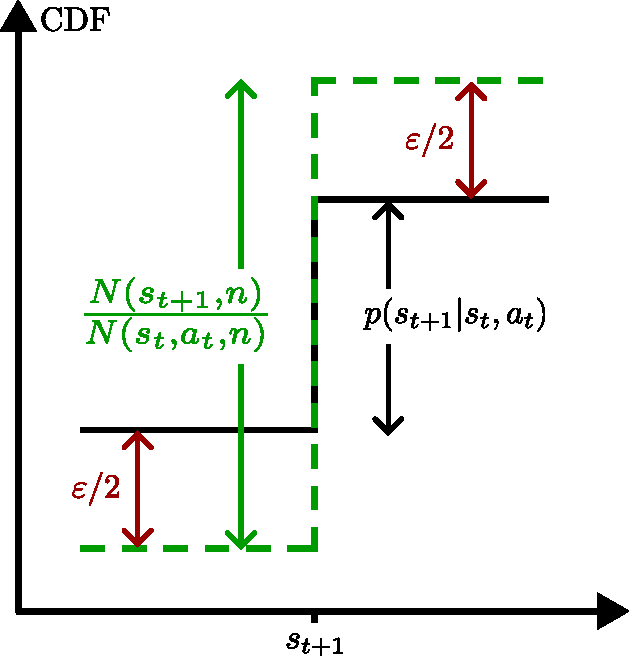
\includegraphics[scale=0.6]{figures/ch4/dkw_diagram.pdf}
        \caption[Bounding the empirical transition probabilities to the true transition probabilities.]{Bounding the empirical transition probabilities to the true transition probabilities. The true cdf is shown as a solid black line, the empirical cdf is shown as a dashed green line, and a worst case error of $\varepsilon/2$, using Theorem \ref{thrm:dkw_inequality}, is shown in red. The probability mass of $p(s_{t+1}|s_t,a_t)$ and empirical probability mass of $\frac{N(s_{t+1},n)}{N(s_t,a_t,n)}$ is also indicated to demonstrate how the constructed distribution gives Corollary \ref{cor:bound_transition_distribution}.}
        \label{fig:dkw_diag}
    \end{figure}







        


    Now that Corollary \ref{cor:bound_transition_distribution} can be used to bound  the empirical transition distribution to the true transition distribution,  a general purpose concentration inequality for Q-values can be proved for use in later proofs.
    
    \begin{lemma} \label{lem:stochastic_step}
        Consider any Boltzmann MCTS process, and some state action pair $(s_t,a_t)\in\cl{S}\times\cl{A}$. Let $\dot{V}^{N(s,n)}(s):\cl{S}\rightarrow \bb{R}$, $\dot{V}^*(s):\cl{S}\rightarrow \bb{R}$ be some estimated and optimal value functions respectively and suppose that for all $s_{t+1}\in\suc{s_t}{a_t}$ that there is some $C_{s_{t+1}}, k_{s_{t+1}}>0$ such that for all $\varepsilon_0 >0$:
        \begin{align}
            \Pr\left(\left| \dot{V}^{N(s_{t+1})}(s_{t+1}) - \dot{V}^*(s_{t+1}) \right| > \varepsilon_0 \right) \leq C_{s_{t+1}}\exp(-k_{s_{t+1}}\varepsilon_0^2 N(s')).
        \end{align}
        
        If the optimal and estimated Q-values are defined as follows: 
        \begin{align}
            \dot{Q}^*(s,a)&=R(s,a)+\bb{E}_{s'\sim p(\cdot|s,a)}\left[\dot{V}^*(s')\right], \\
            \dot{Q}^{N(s,a,n)}(s,a)&=R(s,a)+\sum_{s'\in\suc{s}{a}} \left[
                \frac{N(s',n)}{N(s,a,n)} \dot{V}^{N(s',n)}(s')\right].
        \end{align}
        
        Then there exists some $C,k>0$, for all $\varepsilon>0$ such that:
        \begin{align}
            \Pr\left(\left| \dot{Q}^{N(s,a,n)}(s,a) - \dot{Q}^*(s,a) \right| > \varepsilon \right) \leq C\exp(-k\varepsilon^2 N(s,a,n)).
        \end{align}
    \end{lemma}
    
    \begin{proof}
        By the assumed bounds, Lemma \ref{lem:union_bound} and Lemma \ref{lem:s_to_sa}, there is some $C_1,k_1>0$, such that for any $\varepsilon_1 >0$:
        \begin{align}
            \Pr\left(\forall s_{t+1}. \left|\dot{V}^{N(s_{t+1})}(s_{t+1})-\dot{V}^*(s_{t+1}) \right| \leq \varepsilon_1 \right) > 1-C_1\exp(-k_1\varepsilon_1^2 N(s_t,a_t,n)). \label{local:one}
        \end{align}

        And recall that for any $p(s_{t+1}|s_t,a_t) > \varepsilon_2>0$, using Corollary \ref{cor:bound_transition_distribution} that:
        \begin{align}
            \Pr\left(\max_{s_{t+1}\in\suc{s_t}{a_t}} 
                \left| \frac{N(s_{t+1},n)}{N(s_t,a_t,n)} - p(s_{t+1}|s_t,a_t) \right| 
                \leq \varepsilon_2 \right) 
                    > 1 - 2 \exp\left(-\frac{1}{2}\varepsilon_2^2 N(s_t,a_t,n) \right). \label{local:two}
        \end{align}
        
        If the events in Inequalities (\ref{local:one}) and (\ref{local:two}) hold, then the following inequalities must also hold:
        \begin{align}
            \dot{V}^*(s_{t+1})- \varepsilon_1 
                &\leq \dot{V}^{N_n(s_{t+1},n)}(s_{t+1}) 
                \leq \dot{V}^*(s_{t+1})+ \varepsilon_1 \\
            p(s_{t+1}|s_t,a_t) - \varepsilon_2 
                &\leq \frac{N(s_{t+1},n)}{N(s_t,a_t,n)} 
                \leq p(s_{t+1}|s_t,a_t) + \varepsilon_2.
        \end{align} 
        
        The upper bounds on $\dot{V}^{N_n(s_{t+1},n)}(s_{t+1})$ and $N(s_{t+1},n)/N(s_t,a_t,n)$ can be used to obtain an upper bound on $\dot{Q}^{N(s_t,a_t,n)}(s_t,a_t)$: 
        \begin{align}
            &\dot{Q}^{N(s_t,a_t,n)}(s_t,a_t) \\
                =& R(s_t,a_t) 
                    + \sum_{s_{t+1}\in\suc{s_t}{a_t}}\frac{N(s_{t+1},n)}{N(s_t,a_t,n)} 
                        \dot{V}^{N(s_{t+1},n)}(s_{t+1}) \\
                \leq& R(s_t,a_t) 
                    + \sum_{s_{t+1}\in\suc{s_t}{a_t}}(p(s_{t+1}|s_t,a_t)+\varepsilon_2)
                        (\dot{V}^*(s_{t+1})+\varepsilon_1) \\
                =& R(s_t,a_t) 
                    + \bb{E}_{s_{t+1}\sim p(\cdot|s_t,a_t)}[\dot{V}^*(s_{t+1})] 
                    + \varepsilon_1 
                    + \varepsilon_2\sum_{s_{t+1}\in\suc{s_t}{a_t}} \dot{V}^*(s_{t+1}) 
                    + \varepsilon_1 \varepsilon_2 \\
                \leq& R(s_t,a_t) 
                    + \bb{E}_{s_{t+1}\sim p(\cdot|s_t,a_t)}[\dot{V}^*(s_{t+1})] 
                    + \varepsilon_2\left|\sum_{s_{t+1}\in\suc{s_t}{a_t}} \dot{V}^*(s_{t+1})\right| 
                    + \varepsilon_1 + \varepsilon_1 \varepsilon_2 \\
                =& \dot{Q}^*(s_t,a_t) 
                    + \varepsilon_2\left|\sum_{s_{t+1}\in\suc{s_t}{a_t}} \dot{V}^*(s_{t+1})\right| 
                    + \varepsilon_1 
                    + \varepsilon_1 \varepsilon_2.
        \end{align}
        
        Following the similar reasoning but using the lower bounds on $\dot{V}^{N_n(s_{t+1},n)}(s_{t+1})$ and $N(s_{t+1},n)/N(s_t,a_t,n)$ gives: \todo{There is some special cases when V is negative, having to use the other bound, but the upper and lower bound have a bit of leway which handles all four cases of using plus minus epsilon one and two.}
        \begin{align}
            \dot{Q}^{N(s_t,a_t,n)}(s_t,a_t) 
                &\geq \dot{Q}^*(s_t,a_t) 
                    - \varepsilon_2\left|\sum_{s_{t+1}\in\suc{s_t}{a_t}} \dot{V}^*(s_{t+1})\right| 
                    - \varepsilon_1 
                    - \varepsilon_1 \varepsilon_2.
        \end{align}
        
        Now given an arbitrary $\varepsilon >0$, recalling that $\varepsilon_1,\varepsilon_2>0$ were arbitrary, set $\varepsilon_1 = \varepsilon/3$ and $\varepsilon_2 = \min(\varepsilon/3, \varepsilon/3|\sum_{s_{t+1}} \dot{V}^*(s_{t+1})|)$ to give:
        %
        \begin{align}
            \dot{Q}^*(s_t,a_t) - \varepsilon \leq \dot{Q}^{N(s_t,a_t,n)}(s_t,a_t) \leq \dot{Q}^*(s_t,a_t) + \varepsilon.
        \end{align}
        
        Using Lemma \ref{lem:union_bound} liberally, there is some $C_2,C_3,k_2,k_3>0$ such that:
        \begin{align}
            &\Pr\left(\left| \dot{Q}^{N(s_t,a_t,n)}(s_t,a_t) - \dot{Q}^*(s_t,a_t) \right| \leq \varepsilon \right) \\
                >& \left(1-C_1\exp(-k_1\varepsilon_1^2 N(s_t,a_t,n))\right) 
                    \left(1-2\exp\left(-\frac{1}{2}\varepsilon_2^2 N(s_t,a_t,n) \right)\right) \\
                =& \left(1-C_2\exp(-k_2 \varepsilon^2 N(s_t,a_t,n) \right) 
                    \cdot \left(1-C_3\exp(-k_3 \varepsilon^2 N(s_t,a_t,n)\right) \\
                % =& 1 -C_2\exp(-k_2 \varepsilon^2 N(s_t,a_t,n)) -C_3\exp(-k_3 \varepsilon^2 N(s_t,a_t,n)) \notag \\
                %     &+ C_2C_3\exp(-(k_2+k_3)\varepsilon^2 N(s_t,a_t,n) ) \\
                >& 1 -C_2\exp(-k_2 \varepsilon^2 N(s_t,a_t,n)) -C_3\exp(-k_3 \varepsilon^2 N(s_t,a_t,n)).
        \end{align}
        
        Finally, by negating and setting $C=C_2+C_3$ and $k=\min(k_2,k_3)$ in Lemma \todo{ref} the result follows:
        \begin{align}
                \Pr\left(\left| \dot{Q}^{N(s_t,a_t,n)}(s_t,a_t) - \dot{Q}^*(s_t,a_t) \right| > \varepsilon \right) \leq C\exp(-k\varepsilon^2 N(s_t,a_t,n)).
        \end{align}
    \end{proof}















  
\subsection{MENTS results} \label{app:ments_results}

    This subsection provides results related to MENTS in the setting of that standard reinforcement learning objective. Concentration inequalities are given around the optimal soft values to start with, although this result is similar to soem of the results provided in \cite{ments} \todo{this is still provided to keep this thesis' proofs self contained. (although its not as we use lots of things like hoeffdings, and also use UCT style proofs prsumably later on.) We could say ``to keep the proofs compatible with the other results provided. Or we could just omit it and reference the MENTS paper...''} Afterwards, the concentration inequalities are combined with results about maximum entropy reinforcement learning \todo{ref the section where we did that} to provide bounds on the simple regret of MENTS, given constraints on the temperature.
    








    To prove the concentration inequality around the optimal soft values, start by showing an inductive step.

    
    \begin{lemma} \label{lem:ments_val_induction_step}
        Consider a MENTS process. Let $s_t\in\cl{S}$, with $1\leq t \leq H$ \todo{update for thtspp notation}. If for all $s_{t+1}\in\bigcup_{a\in\cl{A}}\suc{s_t}{a}$ there is some $C_{s_{t+1}},k_{s_{t+1}}>0$ for any $\varepsilon_{s_{t+1}}>0$:
        \begin{align}
            \Pr\left(\left| \mVments{N(s_{t+1},n)}(s_{t+1}) - V_{\sft}^*(s_{t+1}) \right| > \varepsilon_{s_{t+1}} \right) 
                &\leq C_{s_{t+1}}\exp\left( -k_{s_{t+1}}\varepsilon_{s_{t+1}}^2 N(s_{t+1},n) \right), 
        \end{align}
        then there is some $C,k>0$, for any $\varepsilon>0$:
        \begin{align}
            \Pr\left(\left| \mVments{N(s_{t},n)}(s_t) - V_{\sft}^*(s_{t}) \right| > \varepsilon \right) 
                &\leq C\exp\left( -k\varepsilon^2 N(s_{t},n) \right).
        \end{align}
    \end{lemma}
    
    \begin{proof}
        Given the assumptions and by Lemmas \ref{lem:stochastic_step}, \ref{lem:sa_to_s} and \ref{lem:union_bound}, there is some $C,k>0$ such that for any $\varepsilon>0$:
        \begin{align}
            \Pr\left(\forall a_t\in\cl{A}. \left|\mQments{N(s_t,a_t,n)}(s_t,a_t)-Q_{\sft}^*(s_t,a_t)\right|\leq \varepsilon\right) &> 1-C \exp(-k \varepsilon^2 N(s_t,n)).
        \end{align}
        
        So with probability at least $1-C \exp(-k \varepsilon^2 N(s_t,n))$, for any $a_t$, the following holds:
        \begin{align}
            Q_{\sft}^*(s_t,a_t) - \varepsilon \leq \mQments{N(s_t,a_t,n)}(s_t,a_t) \leq Q_{\sft}^*(s_t,a_t) + \varepsilon. 
        \end{align}
        
        Using the upper bound on $\mQments{N(s_t,a_t,n)}(s_t,a_t)$ in the soft backup equation for $\mVments{N(s_t,n)}(s_t)$ (Equation (\ref{appeq:soft_v_backup}) gives:
        \begin{align}
            \mVments{N(s_t,n)}(s_t) &= \alpha \log \sum_{a\in\cl{A}} 
                    \exp\left(\frac{\mQments{N(s_t,a_t,n)}(s_t,a_t)}{\alpha}\right) \\
                &\leq \alpha \log \sum_{a\in\cl{A}} \exp\left(\frac{Q_{\sft}^*(s_t,a_t)+\varepsilon}{\alpha}\right) \\
                &= \left[\alpha \log \sum_{a\in\cl{A}} \exp\left(\frac{Q_{\sft}^*(s_t,a_t)}{\alpha}\right)\right] 
                    + \varepsilon \\
                &= V_{\sft}^*(s_t) + \varepsilon,
        \end{align}
        noting that the \textit{softmax} function monotonically increases in its arguments. Then with similar reasoning using the lower bound on $\mQments{N(s_t,a_t,n)}(s_t,a_t)$ gives:
        \begin{align}
            \mVments{N(s_t,n)}(s_t) \geq V_{\sft}^*(s_t) - \varepsilon,
        \end{align}
        and hence:
        \begin{align}
            |\mVments{N(s_t,n)}(s_t)-V_{\sft}^*(s_t)| \leq \varepsilon.
        \end{align}
        
        This therefore shows: \todo{some comment about how if A implies B then pr(B) more than pr(A)}
        \begin{align}
            \Pr\left(\left|\mVments{N(s_t,n)}(s_t)-V_{\sft}^*(s_t)\right| \leq \varepsilon_1\right) > 1-C \exp(-k \varepsilon^2 N(s_t,n)),
        \end{align}
        and negating probabilities gives the result.
    \end{proof}









        
    
    Then completing the induction gives the concentration inequalities desired for any state that MENTS might visit.
    \begin{theorem} \label{thrm:ments_val_converge}
        Consider a MENTS process, let $s_t\in\cl{S}$ then there is some $C,k>0$ for any $\varepsilon>0$:
        \begin{align}
            \Pr\left(\left| \mVments{N(s_{t},n)}(s_{t}) - V_{\sft}^*(s_{t}) \right| > \varepsilon \right) 
                &\leq C\exp\left( -k\varepsilon^2 N(s_{t},n) \right).
        \end{align}
        Moreover, at the root node $s_0$:
        \begin{align}
            \Pr\left(\left| \mVments{N(s_{0},n)}(s_{0}) - V_{\sft}^*(s_{0}) \right| > \varepsilon \right) 
                &\leq C\exp\left( -k\varepsilon^2 n \right). \label{local:three}
        \end{align}
        And hence $\mVments{N(s_{t},n)}(s_{t}) \rap V_{\sft}^*(s_{t})$.
    \end{theorem}
    \begin{proof}
        Consider that the result holds for $t=H+1$, because $\mVments{N(s_{H+1},n)}(s_{H+1})=V_{\sft}^*(s_{H+1})=0$. Therefore the result holds for any $t=0,...,H+1$ by induction using Lemma \ref{lem:ments_val_induction_step}. Noting that $N(s_0)=n$ gives (\ref{local:three}). \todo{To see the convergence in probability, let }$n\rightarrow\infty$. \todo{Double check the H stuf is consistent with the thtspp and MDP defns}
    \end{proof}










    Provided MENTS's temperature parameter is set small enough, such that the optimal standard and soft values lead to identical recommendation policies \todo{ref the max entropy proof of this}, then MENTS is consistent and the expected simple regret tends to zero exponentially. This is shown in the following lemma.
        
    \begin{lemma} \label{lem:ments_imm_simple_regret}
        Consider a MENTS process with $\alpha<\Delta_{\cl{M}}/3H\log |\cl{A}|$. Let $s_t\in\cl{S}$, with $1\leq t \leq H$ then there is some $C',k'>0$ such that:
        \begin{align}
            \bb{E} \sreg(s_{t},\mpsiments{n}) &\leq C'\exp\left( -k' N(s_{t},n) \right).
        \end{align}
    \end{lemma}
    \begin{proof}
        \todo{Why cant we just replace this with, the values converge in probability from the previous result, and then use that it means the recommendation policy converges in probability, and then use that to say simple regret go zero? The case where it doesnt work is if there is suboptimal soft value which equals the optimal soft value (which has no entropy), in this case, becase we need the value ESTIMATES to converge, not the optimal values, we need the temperature to be a bit stricter. I think}

        Let $a^*$ be the optimal action with respect to the soft values, so $a^*=\argmax_{a\in\cl{A}} Q_{\sft}^*(s_t,a)$. Then by Lemma \ref{lem:soft_standard_consistent_order} $a^*$ must also be the optimal action for the standard Q-value function $a^*=\argmax_{a\in\cl{A}} Q^*(s_t,a)$. By Theorem \ref{thrm:ments_val_converge} and Lemmas \ref{lem:stochastic_step} and \ref{lem:sa_to_s} there exists $C_1,k_1>0$ such that for all $\varepsilon_1>0$: \todo{reword this paragraph, its a bit meh}
        \begin{align}
            \Pr\left(\forall a_t\in\cl{A} \left|\mQments{N(s_t,a_t,n)}(s_t,a_t)-Q_{\sft}^*(s_t,a_t)\right|\leq \varepsilon_1\right) &> 1-C_1 \exp(-k_1 \varepsilon_1^2 N(s_t,n)).
        \end{align}
        
        Setting $\varepsilon_1=\Delta_{\cl{M}}/3H\log |\cl{A}|$ then gives with probability at least $1-C_1 \exp(-k_2N(s_t,n))$ (where $k_2=k_1\left(\frac{\Delta_{\cl{M}}}{3H\log|\cl{A}|}\right)^2$) that for all actions $a_t\in\cl{A}$:
        \begin{align}
            Q_{\sft}^*(s_t,a_t) - \Delta_{\cl{M}}/3 \leq \mQments{N(s_t,a_t,n)}(s_t,a_t) \leq Q_{\sft}^*(s_t,a_t) + \Delta_{\cl{M}}/3.
        \end{align}
        
        And hence, with probability at least $1-C_1 \exp(-k_2N(s_t,n))$, for all $a\in\cl{A}-\{a^*\}$ we have:
        \begin{align}
            \mQments{N(s_t,a,n)}(s_t,a)
                \leq& Q_{\sft}^*(s_t,a) + \Delta_{\cl{M}}/3 \\
                \leq& Q^*(s_t,a) + \alpha H\log |\cl{A}| + \Delta_{\cl{M}}/3 \\
                \leq& Q^*(s_t,a) + 2\Delta_{\cl{M}}/3 \\
                \leq& Q^*(s_t,a^*) - \Delta_{\cl{M}}/3 \\
                \leq& Q_{\sft}^*(s_t,a^*) - \Delta_{\cl{M}}/3 \\
                \leq& \mQments{N(s_t,a^*,n)}(s_t,a^*). \label{local:nine}
        \end{align}
        
        Where in the above, the first line holds from the upper bound on $\mQments{N(s_t,a_t,n)}(s_t,a_t)$; The second holds from maximising the standard return and entropy portions of the soft value separately (recall Inequality (\ref{appeq:softdiv}) in Lemma \ref{lem:soft_standard_consistent_order}); The third holds from the assumption on $\alpha$; The fourth holds from the definition of $\Delta_{\cl{M}}$ (also see Inequality (\ref{appeq:delta_diff})); The fifth holds from the optimal soft value being greater than the optimal standard value (Lemma \ref{lem:soft_geq_standard}); And the final line holds by using the lower bound on $\mQments{N(s_t,a_t,n)}(s_t,a_t)$ given above with $a_t=a^*$. 
        
        Negating the probability that (\ref{local:nine}) holds gives:
        \begin{align}
            \Pr\left(\exists a_t\in\cl{A}-\{a^*\}.\left( 
                \mQments{N(s_t,a)}(s_t,a) > \mQments{N(s_t,a^*,n)}(s_t,a^*)\right)\right)
                \leq C_1 \exp(-k_2N(s_t)).
        \end{align}
        
        The expected immediate regret can be bounded as follows:
        \begin{align}
            & \bb{E}\ireg(s_t,\mpsiments{n})  \\
                =& \sum_{a\in\cl{A}-\{a^*\}} 
                    \left(V^*(s_t)-Q^*(s_t,a)\right) \Pr\left(\mpsiments{n}(s_t) =a \right) \\
                =& \sum_{a\in\cl{A}-\{a^*\}} 
                    \left(V^*(s_t)-Q^*(s_t,a)\right) \Pr\left(a = \argmax_{a'} \mQments{N(s_t,a')}(s_t,a') \right) \\
                \leq& \sum_{a\in\cl{A}-\{a^*\}} 
                    \left(V^*(s_t)-Q^*(s_t,a)\right) \Pr\left(\mQments{N(s_t,a,n)}(s_t,a) > \mQments{N(s_t,a^*,n)}(s_t,a^*)  \right) \\
                \leq&  \sum_{a\in\cl{A}-\{a^*\}} 
                    \left(V^*(s_t)-Q^*(s_t,a)\right) C_1 \exp(-k_2N(s_t,n)),
        \end{align}
        where $k'=k_2$ and $C'=C_1\sum_{a\in\cl{A}-\{a^*\}} \left(V^*(s_t)-Q^*(s_t,a)\right)$. Finally, using \todo{ref lemma} gives the result.
    \end{proof}






    


    \todo{HERE HERE HERE HERE HERE}












    %%%%
    % THEORY - Consistency Of Boltzmann MCTS Processes
    %%%%
    
    \subsection{Consistency Of Boltzmann MCTS Processes}

        Because the search temperature is now decayed, we need to show that the exploration term in the search policies leads to actions being sampled infinitely often.


        \todo{This lemma restated means that Boltzmann search policies will select all actions infinitely often.}
        \todo{Check the variables in this proof are consistent with the definitions of N(s,a,m) etc}

        \begin{lemma} \label{lem:inf_often_action_select}
            Let $\rho^m$ be an arbitrary policy, and the following policy: \todo{handle when epsilon is greater than one? I think its just let ell be large enough argument}
            \begin{align} 
                \pi^m(a)=(1-\lambda(m))\rho^m(a) + \lambda(m) \frac{1}{|\cl{A}|}, \label{appeq:ioas_policy}
            \end{align} 
            with $\lambda(m)=\min(1,\epsilon/\log(e+m))$, where $\epsilon\in(0,\infty)$. Let $a^m\sim \pi^m$ be the $m$th sampled action, and let $M(a,m)$ be the number of times action $a$ was selected in the first $m$ samples, i.e. $M(a,m)=\sum_{m=1}^m \one[a^m=a]$. Then for all $a\in\cl{A}$ we have $M(a,m)\raas\infty$ as $m\rightarrow \infty$.
        \end{lemma}
        \begin{proof}
            First consider that if $M(a,m)\not\rightarrow\infty$ then it is logically equivalent to say that there exists some $\ell$ such that from $a^\ell$ onwards that there is some action which is never sampled again. To prove the result, argue by contradiction, and suppose that there is some $\ell\in\bb{N}$ and $b\in\cl{A}$ such that:
            \begin{align}
                \Pr\left(\bigcap_{m=\ell}^\infty a^m \neq b\right) > 0. \label{appeq:ioas_contradict}
            \end{align}

            However, from the definition of equation (\ref{appeq:ioas_policy}) it must be that:
            \begin{align}
                \Pr\left(a^m = b\right) \geq \frac{\lambda(m)}{|\cl{A}|} = \frac{\epsilon}{|\cl{A}| \log(e+m)}.
            \end{align} 

            And so using this lower bound to work out the probability of never sampling action $b$ again after the first $\ell-1$ samples gives:
            \begin{align}
                \Pr\left(\bigcap_{m=\ell}^\infty a^m \neq b \right)
                    &= \lim_{k\rightarrow\infty} \prod_{m=\ell}^k 
                        \Pr(a^m \neq b) \\
                    &\leq \lim_{k\rightarrow\infty} \prod_{m=\ell}^k 
                        \left( 1 - \frac{\epsilon}{|\cl{A}|\log(e+k)} \right) \\
                    &\leq \lim_{k\rightarrow\infty} 
                        \left( 1 - \frac{\epsilon}{|\cl{A}|\log(e+k)} \right)^{k-\ell} \label{appeq:ioas_one} \\
                    &= 0, \label{appeq:ioas_two}
            \end{align}
            %
            which is in contradiction to inequality (\ref{appeq:ioas_contradict}) that was assumed. Inequality (\ref{appeq:ioas_one}) holds because the factors in the product are increasing with respect to $m$. To see why the final limit equality (\ref{appeq:ioas_two}) holds, consider the simpler function $f(x)=\left(1-1/\log(x)\right)^x$. Taking logarithms and applying L'Hopital's rule \todo{cite?} generously gives:
            \begin{align}
                \lim_{x\rightarrow \infty} \log f(x) 
                &= \lim_{x\rightarrow \infty} x \log\left(1-\frac{1}{\log(x)}\right) \\
                &= \lim_{x\rightarrow \infty} \frac{\log\left(1-\frac{1}{\log(x)}\right)}{x^{-1}} \\
                &= \lim_{x\rightarrow \infty} \frac{\frac{1}{x\log(x)(\log(x)-1)}}{-x^{-2}} \\
                &= \lim_{x\rightarrow \infty} \frac{-x}{\log(x)(\log(x)-1)} \\
                &= \lim_{x\rightarrow \infty} \frac{-x}{2\log(x)-1} \\
                &= \lim_{x\rightarrow \infty} \frac{-x}{2} \\
                &= -\infty.
            \end{align} 
            %
            And thus $\lim_{x\rightarrow\infty} f(x) = \lim_{y\rightarrow -\infty} e^{y} = 0$.

            \todo{cut this down maybe, its a little excessive showing all of the working out?}

            Hence, by contradiction, it must be the case that $\Pr(M(a,m)\not\rightarrow\infty) = 0$, or rather that $\Pr(M(a,m)\rightarrow\infty) = 1$ which is the desired result.
        \end{proof}
        %
        \todo{Can we also say that if its (1 - 1/o(x)) to the x, then it will generally hold, so x to the power of 0.99 could equally be used. And also any polynomial of log(x) could be used} 

        


        \todo{Words about the consequences of this lemma?}

        In direct consequence of Lemma \ref{lem:inf_often_action_select}, every reachable state (and state-action pair) will be visited infinitely often in a Boltzmann MCTS Process.

        \begin{corollary} \label{cor:inf_often_action_select}
            For any Boltzmann MCTS Process (i.e. a MCTS algorithm using a search policy of the form $\pi^m(a)=(1-\lambda(m))\rho^m(a) + \lambda(m) \frac{1}{|\cl{A}|}$), all reachable states from the root node are visited infinitely often. Specifically, for any reachable $s\in\cl{S}$ is must be that $N(s,m)\raas\infty$ and $N(s,a,m)\raas\infty$ as $m\rightarrow\infty$. \todo{handle reachability somewhere better? just make some assumption at the start of the theory section saying we assume all s are reacahable?}
        \end{corollary}
        \begin{proofoutline}
            This is a direct consequence of Lemma \ref{lem:inf_often_action_select} when applied inductively at each node.
        \end{proofoutline}




        \todo{Values in BTS and DENTS converge to V* (Dynamic Programming)}




        \todo{Values in AR-BTS and AR-DENTS converge to V* (and what conditions need to be)}




        \todo{Simple regrets. (Consequence from visit counts tending to infinity, and therefore policy converges)}


        \todo{Theorem that show that values in AR-BTS and AR-DENTS converge}





        \todo{Theorem that shows if backups converge to the optimal, then guaranteed to converge and simple regret tends to 0 which is the result.}


        \todo{Theorem to show that most visited policy will also converge. Say that from the point of values converging it will add exp many additional trials for the. Essentially, if converges after K trials, then each action visited M(a) many times is a constant start. And then N(a) eq new(a) plus M(a) will converge by law of large numbers, and should do exp fast. Basically need to do some DKW and (strong?) law of large numbers stuff. Its just a bit bothersome because the sum is not identically distributed, as each action sampled from a diff distribution.} \todo{also see this llm chat: https://chatgpt.com/c/67ad143f-6374-8007-9126-e90eb9f42578 - I like the argument } \todo{I liked the argument that if xn converges to x then avg(x1,...,xm) also converges to x. I also like how I posed the question to llm}

        %https://en.wikipedia.org/wiki/Dvoretzky%E2%80%93Kiefer%E2%80%93Wolfowitz_inequality
        %https://en.wikipedia.org/wiki/Law_of_large_numbers













    %%%%
    % THEORY - FIRST THING PROOV IN NEURIPS PAPERS
    %%%%










    
    






\section{Full Results}
\label{sec:4-6-fullresults}

    \todo{there's a lot of figures for the D-chain environment, work out how to best fit them in? Or put them in this seperate section?}